
\documentclass[conference]{IEEEtran}
\IEEEoverridecommandlockouts
% The preceding line is only needed to identify funding in the first footnote. If that is unneeded, please comment it out.
\usepackage{cite}
\usepackage{amsmath,amssymb,amsfonts}
\usepackage{algorithmic}
\usepackage{graphicx}
\usepackage{textcomp}
\usepackage{xcolor}
\def\BibTeX{{\rm B\kern-.05em{\sc i\kern-.025em b}\kern-.08em
    T\kern-.1667em\lower.7ex\hbox{E}\kern-.125emX}}
\usepackage{booktabs}
\usepackage{fancyhdr}
\pagestyle{fancy}
\fancyhf{} 
\rfoot{\thepage}
\renewcommand{\headrulewidth}{0pt}
\begin{document}

\title{Capstone Report of Autodrone for Person Re-Identification\\

}

\author{\IEEEauthorblockN{Zening Li, Luxi Zhu, Yanlin Jin, Xiangxin Wan, Michael Chiu, Jiaer Xia}
\affil{\textit {\{zl156, lz70, yj56, xw83, mc202, jx37\}@rice.edu}}
\IEEEauthorblockA{School of Electrical and Computer Engineering}
\IEEEauthorblockA{Rice University, Houston, TX 77005 USA}

}


\maketitle

\begin{abstract}

This project outlines developing an autonomous drone system designed for first responders working in hazardous environments. It details advancements in hardware, such as a 360-degree camera, and software, particularly in object detection algorithms like YOLOv9 optimized for real-time performance. Additionally, it includes 3D reconstruction capabilities using Gaussian splatting and LiDAR data integration, enhancing environmental modeling accuracy. The integration of these technologies into ROS2 enhances operational simulations and real-world applications, highlighting the drone's potential to improve safety and efficiency in emergency responses. The system continues to evolve, focusing on refining its capabilities for reliable use in diverse conditions.
\end{abstract}


\section{Introduction}
Customized drones provide a wide range of utilities through diverse capabilities tailored to meet the users needs. One commonality across various configurations is that it provides some degree of separation between the user and where the drone is operating. This is particularly useful when working in hazardous environments, like the ones first responders often find themselves. First responders place themselves in danger in situations where they are looking for people in emergency situations like building fires or search and rescue. 

A drone capable of navigating harsh environments that can detect people not only improve their chances of survival by getting help to them sooner but it also protects the first responders by keeping them removed from the dangerous environment until they have more information. To do so, the drone needs to fly autonomously, detect people or other objects through sensors, map or provide imagery, and wirelessly communicate this back in real time or near real time. 

To accomplish this, we focused on methods for hardware to support an autonomous drone, 5G connectivity, computer vision object detection, and 3D Reconstruction. The ability to simultaneously fit on the drone during the flight physically constrain the implementation of these solutions. In this paper, we will discuss the methods and results achieved in each of these four domains. 


\section{Methods}

\subsection{Hardware}
\subsubsection{General introduction}
\begin{figure}[h]
    \centering
    {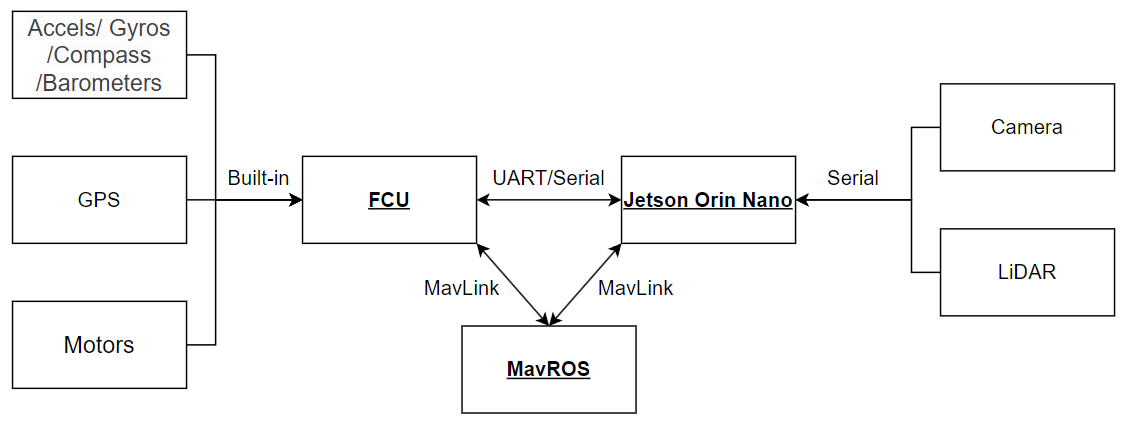
\includegraphics[scale=0.3]{figures/flowchart.png}}
    \caption{System Flowchart of the Drone}
    \label{Stepper Motor}
\end{figure}
\begin{figure}[ht]
    \centering
    \begin{minipage}{0.24\textwidth}
        \centering
        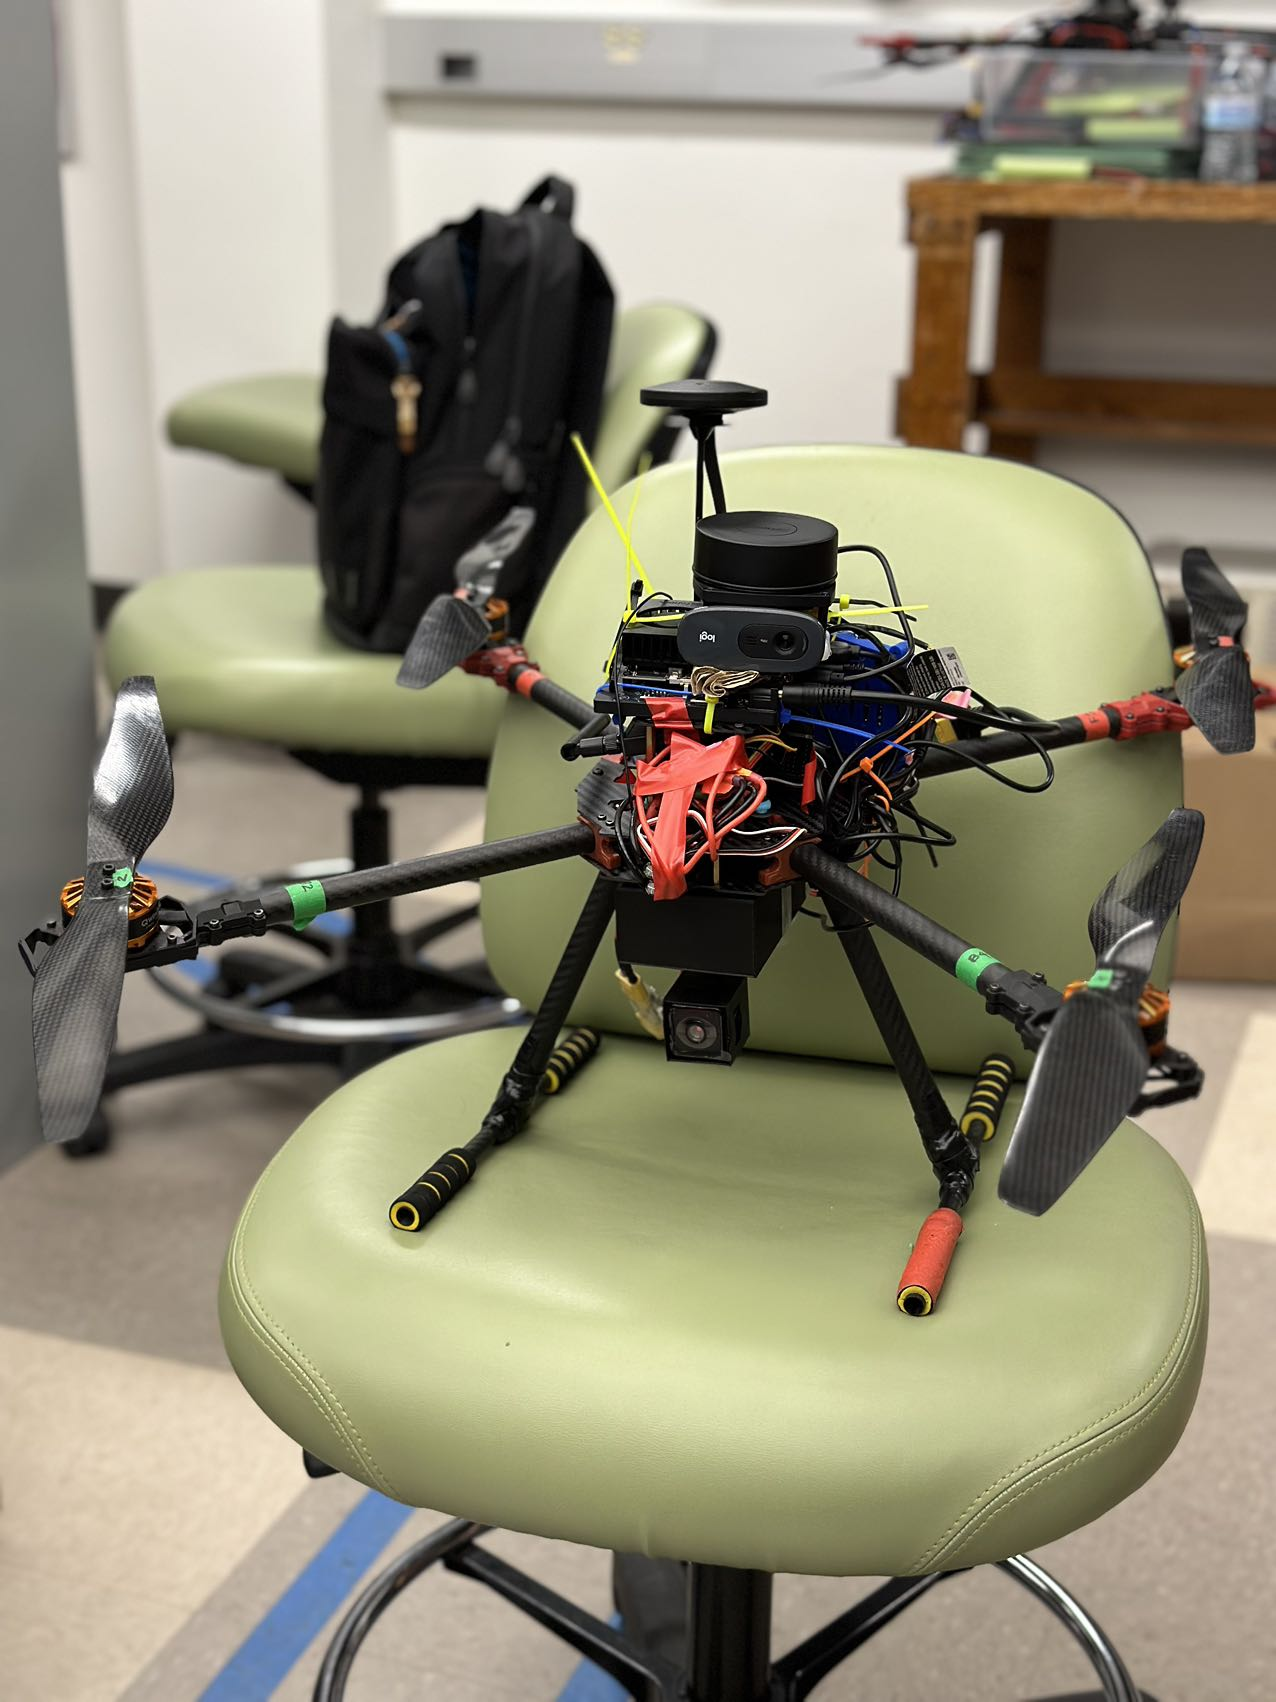
\includegraphics[width=0.8\linewidth]{figures/drone_all.png}
        \caption{All Equipped Drone}
        \label{All Equipped Drone}
    \end{minipage}
    \hfill
    \begin{minipage}{0.24\textwidth}
        \centering
        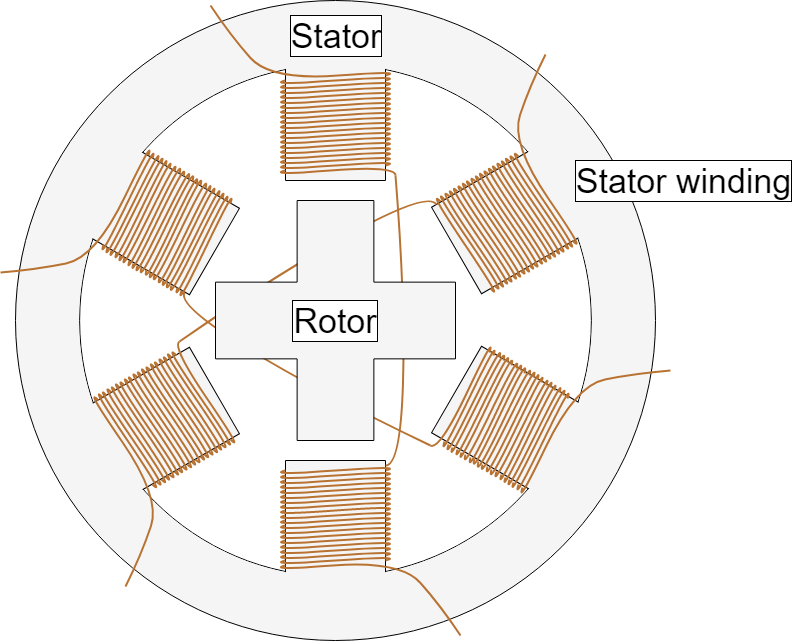
\includegraphics[width=\linewidth]{figures/stepper_motor.png}
        \caption{Stepper Motor Interface Diagram}
        \label{Stepper Motor}
    \end{minipage}
\end{figure}
In the AutoDrone project, our system comprises two primary devices: the Jetson Orin Nano and the Flight Control Unit (FCU). FCU is equipped with various sensors, including gyroscopes, accelerometers, and temperature meters, and it also manages GPS input and power distribution to the motor.
Our main controller is the Jetson Orin Nano, which is essential for executing tasks. It captures images from the camera and LiDAR, applying deep learning algorithms for accurate person re-identification and tracking. These algorithms process depth information, guiding the drone’s
flight controller for precise maneuvering in complex environments.
Our project utilizes two embedded devices: the GPU-equipped Jetson Orin Nano. We are testing both to assess their compatibility and effectiveness for the project, ensuring optimal performance in real-world scenarios.

% \begin{figure}[h]
%     \centering
%     {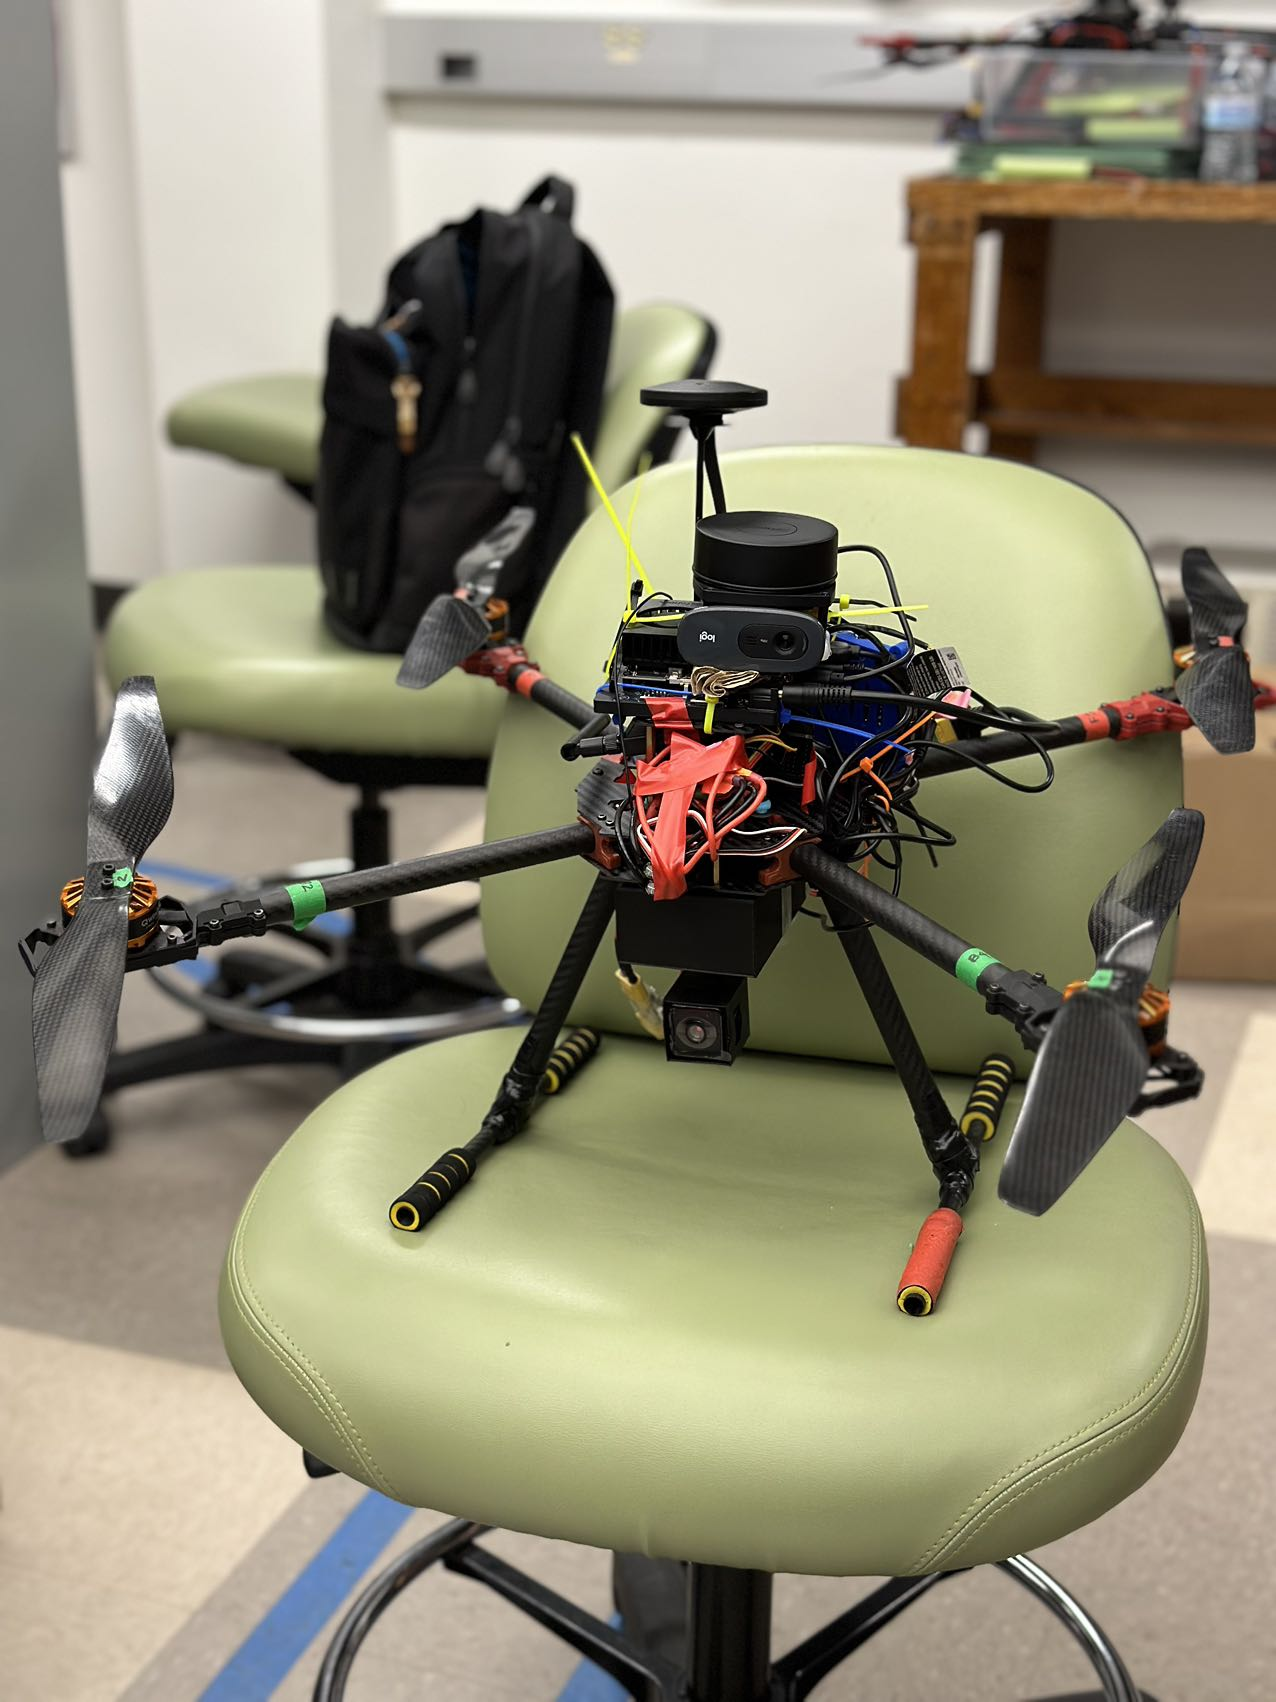
\includegraphics[scale=0.08]{figures/drone_all.png}}
%     \caption{All Equipped Drone}
%     \label{Stepper Motor}
% \end{figure}

\subsubsection{360-degree real-time rotational camera
} 
The 360-degree real-time rotational camera system is a sophisticated addition to our autodrone, designed to provide operators with a comprehensive, live view of the drone's surroundings. This innovative feature consists of a stepper motor and a wireless transmission camera, strategically mounted beneath the drone's battery compartment.

Stepper motors are a type of brushless DC motor that can precisely control angular position, speed, and direction. They are widely used in applications requiring accurate positioning, such as robotics, CNC machines, and in this case, the 360-degree rotational camera system for our autodrone.

Principles of Stepper Motors:

1. Construction: Stepper motors consist of a rotor (permanent magnet) and a stator (electromagnets). The stator has multiple windings that can be energized in a specific sequence to create a rotating magnetic field, causing the rotor to rotate in precise increments, or "steps."\cite{stepper}
2. Step Angle: The step angle is the amount of rotation the motor shaft undergoes for each step. It is determined by the number of teeth on the rotor and the number of stator windings. Common step angles include 0.9°, 1.8°, and 7.5°, with smaller step angles providing higher resolution and accuracy.\\
% \begin{figure}[h]
%     \centering
%     {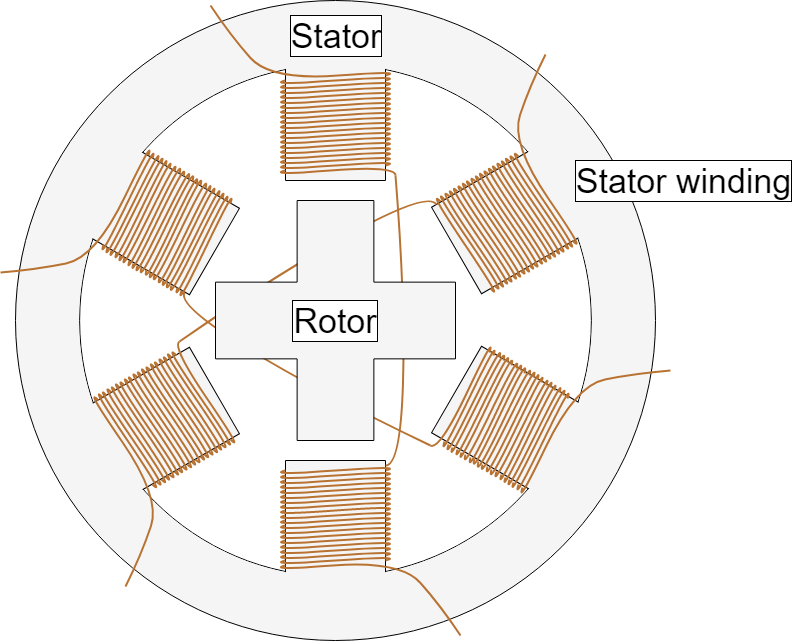
\includegraphics[scale=0.2]{figures/stepper_motor.png}}
%     \caption{Stepper Motor Interface Diagram}
%     \label{Stepper Motor}
% \end{figure}
3. Driver Circuits: Stepper motors require a driver circuit to control the sequence and timing of the energizing of the stator windings\ref{Stepper Motor}. The driver circuit receives step and direction signals from a controller, such as a microcontroller or Raspberry Pi, and translates them into the appropriate sequence of pulses to drive the motor.

The stepper motor, known for its precision and reliability, is connected to the control lines of the Raspberry Pi, a compact single-board computer. This connection allows operators to remotely control the rotation of the camera using a laptop via SSH (Secure Shell) to access the Raspberry Pi. By sending appropriate commands to the Raspberry Pi, the stepper motor can be instructed to rotate the camera in precise increments, enabling a seamless 360-degree view of the drone's environment\cite{rasp}.

% 1. GPIO Pins: Assign the appropriate GPIO pins on the Raspberry Pi to control the driver module. Typically, you'll need to connect the driver module's step, direction, and enable pins to the corresponding GPIO pins on the Raspberry Pi.

% 2. Software Control: Use a programming language like Python to control the stepper motor. Popular libraries such as RPi.GPIO and pigpio provide convenient functions for setting up and controlling the GPIO pins\cite{rasp}.

% 3. Pulse Generation: To rotate the stepper motor, generate a series of pulses on the step pin of the driver module. The frequency and number of pulses determine the speed and distance of rotation, respectively. Use appropriate timing functions, such as time.sleep() or pigpio's wave functions, to control the pulse timing.

% 4. Direction Control: Set the direction pin to either HIGH or LOW to control the direction of rotation. Changing the state of the direction pin will cause the motor to rotate in the opposite direction.

% 5. Microstepping: our driver modules support microstepping, which allows for finer control of the stepper motor's position. By configuring the driver module and sending a signal from the Raspberry Pi with an interval of 0.03 seconds, we can achieve higher resolution and smoother motion.

The wireless monitoring camera is a compact, off-the-shelf unit that comes with built-in transmission functionality. This plug-and-play feature simplifies the implementation process, as it eliminates the need for complex wiring or additional transmission modules. The camera captures high-quality video footage and transmits it wirelessly to the operator's laptop or control station in real-time.
 

\subsection{Wireless}
\subsubsection{Environment}
Testing focused primarily on using a 5G modem by Sixfab that offered a small form factor system using a Quectel RM502Q-AE module. A RM520N-GL module was also used for testing and comparison of configuration parameters for connecting to the network. We also made use of two host environments. The target working environment is the Jetson Nano mounted on drone but a Linux VM (Ubuntu 20.04.6 LTS) was also used for the ease and availability during testing. Our project makes use of a separate project at Rice University that works towards implementing a 5G network using OpenAir implementation for an Nvidia Base Station. Initial User Equipment (UE) testing on the local implementation used an Android cell phone.
\subsubsection{Software}
The first stage worked to integrate the host with the UE. Key components to install were USB Serial Driver, ATCOM, minicom, and Quectel QConnectManager (QCM) with related drivers. The USB Serial Driver enables the host OS to interact with the module. ATCOM is the command series for configuring and manipulating the module. Minicom is not directly necessary but it provides a text based interface for sending AT Commands and receiving the output from the module. Last, QCM establishes the Network Interface for the module to use when establishing the Data Session with the 5G Network. Two possible drivers to use with QCM are QMI WWAN or GobiNet. On both host environemnts, we used QCM v1.6.2. During the majority of testing, we used the QMI WWAN Driver v1.2.1. Due primarily to differences in architecture and kernel, on the Nano we used GobiNet v1.6.3. When installing, a small modification to one of the source files was necessary in order to compile using the AARCH64 instead of the x86\_64 architecutre in the test environment. 
\subsubsection{UE Configuration}
To configure the SIM Card, we used an OpenCell SIM and their software UICC v3.4. For our implemenation, we were able to duplicate OpenAir SIM parameters with modifications to the IMSI to deconflict between the three devices we used. To configure the RM502 and RM520, we used AT Commands. AT+CGDCONT=1,"IP","oai","0.0.0.0",0,0,0,0 sets the specifc parameters for establishing a data session after registering on the network. During testing, we made use of other commands that allowed us to restrict operating modes such as 5G Standalone (SA) versus 5G Nonstandalone (NSA) or restricting to specific bands for debugging purposes. We also verified that the default settings fit the parameters of the 5G network we were testing with. Additionally, for the RM502 module, we had to change a default setting using AT+QCFG="usbnet",0 in order to allow the QCM to create the interface with the module. 

\subsection{Object Dectection}
\subsubsection{Dataset Choice}
The VisDrone Dataset\cite{visdrone} serves as an extensive benchmark aimed at advancing drone-based image and video analysis. This dataset is particularly suited for research due to its use of drone-mounted cameras, which capture diverse conditions. The focus of the dataset is on 10 vehicle classes, encompassing a variety of scenarios such as sparse and densely populated areas, under varying weather and lighting conditions. These features make the VisDrone Dataset a robust tool for developing and testing advanced analytic techniques in the field of drone-operated imaging.

\subsubsection{Object Detection Algorithms}

Various object detection algorithms, including FasterRCNN \cite{FasterRCNN}, RetinaNet \cite{RetinaNet}, YOLOv5 \cite{YOLOv5}, YOLOv8 \cite{YOLOv8}, and YOLOv9 \cite{YOLOv9}, were implemented and studied within the project. These methods encompass both single-stage and two-stage detectors. While Faster RCNN operates as a two-stage detector by proposing regions via a Region Proposal Network (RPN) and then refining those proposals with a separate detection network, RetinaNet and the YOLO family serve as single-stage detectors, performing localization and classification in a single pass.

RetinaNet employs dense sampling across an image pyramid and introduces focal loss to tackle class imbalance during training, while the YOLO family partitions the input image into a grid for bounding box, confidence score, and class probability predictions within each grid cell. YOLOv8 specifically focused on improving performance and accuracy through techniques like model pruning, hyperparameter evolution, and better augmentation pipelines compared to YOLOv5. YOLOv9, a recently released real-time object detector, introduces Programmable Gradient Information (PGI) to mitigate information loss in deep networks and utilizes a lightweight Generalized Efficient Layer Aggregation Network (GELAN) architecture, claiming superior parameter utilization compared to state-of-the-art methods. 

To evaluate the accuracy and speed of these algorithms for potential deployment on autodrones, RetinaNet, YOLOv8, and YOLOv9 were trained and tested on the VisDrone dataset using an NVIDIA A100 GPU. This dataset offers a diverse range of over 265,000 images captured by drones across multiple cities in China, enabling comprehensive evaluation in various urban scenarios.

\subsubsection{Integration into ROS2 for Simulation}
Following algorithm selection, integration into the Robot Operating System 2 (ROS2) for simulation purposes ensued. YOLOv9 and YOLOv8 were implemented within ROS2, facilitating real-time object detection simulations using a flying drone in Gazebo. The simulation environment was established using ROS2 Humble and Gazebo Garden on Ubuntu 22.04, with PX4 Autopilot employed for model development. To compare the performances of YOLOv9 and YOLOv8 in this simulated setting, a scenario featuring one person and three cars was constructed. Manual control of the drone was achieved using a virtual joystick, with the algorithms tested on real-time images captured by the drone's camera. The testing interface is shown in Figure \ref{interface}. Further performance analysis involved comparative speed assessments of YOLOv9 and YOLOv8 on different hardware configurations, including an Intel Core i7 CPU and an Nvidia GeForce RTX 3070 GPU. These evaluations provided insights into the algorithms' inference times, informing the determination of the most suitable algorithm for real-time object detection on the autodrone platform.

\begin{figure}[htbp]
    \centering
    \resizebox{9cm}{5cm}
    {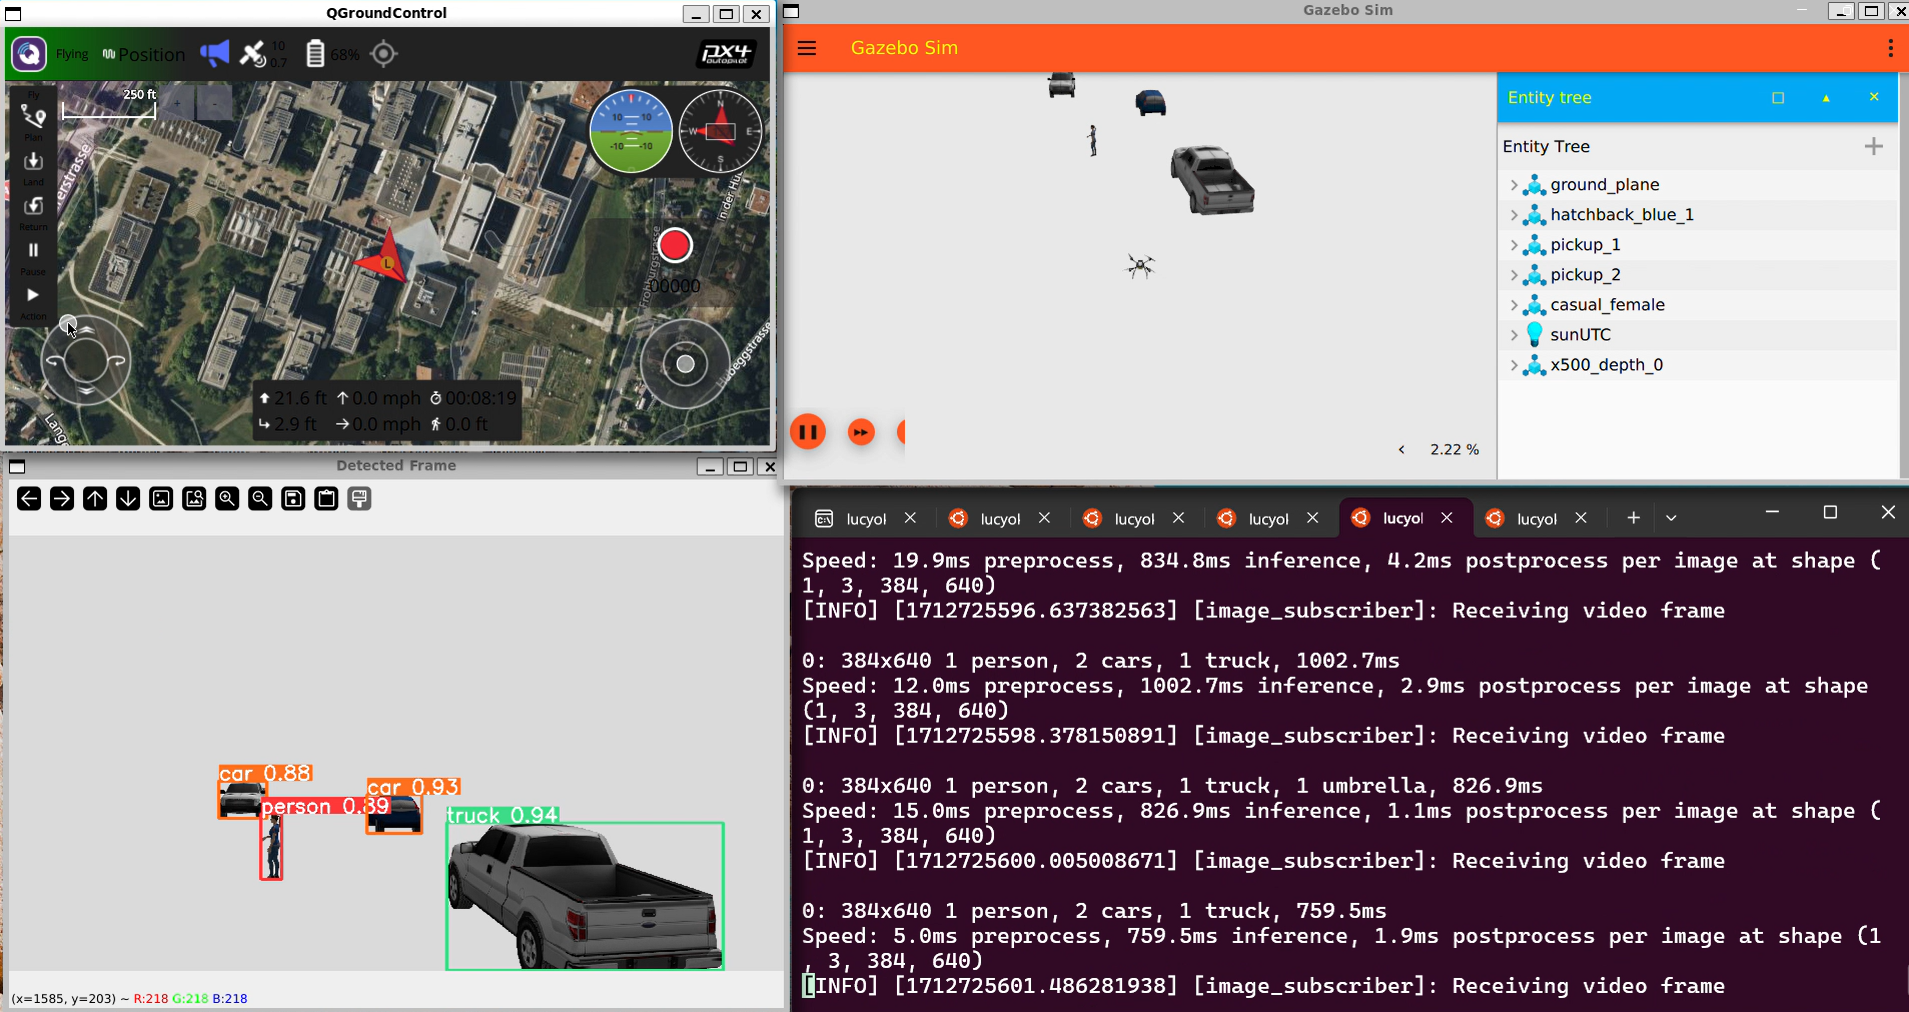
\includegraphics{figures/gazebo_simulation_interface.png}}
    \caption{Simulation Testing Interface}
    \label{interface}
\end{figure}
\subsubsection{Deployment on Nvidia Jetson Orin Nano}

To deploy on the Jetson Orin Nano, begin by flashing the device with Ubuntu 22.04 as the operating system, using NVIDIA SDK Manager. The current SDK version is 6.0, as of April 2, 2024, and it requires at least 50GB of storage space. Once the device is set up, proceed with installing the necessary packages. For a setup without Docker, the Ultralytics Package along with PyTorch and Torchvision need to be installed directly into the environment, which can be a tedious process if incompatible packages are encountered, often leading to failures. Alternatively, using the l4t-pytorch Docker image is recommended as it comes preloaded with PyTorch and Torchvision within a Python environment, facilitating a smoother installation process.
\subsection{3D Reconstruction}
\subsubsection{Gaussian Splatting}
% As a novel way to explicitly represent the 3D scene, Gaussian Splatting has become increasingly popular recently.
Gaussian splatting \cite{3dgs} explicitly represent the 3D scene with millions of 3D Gaussians and enables fast rendering by projecting gaussians onto image plane through differentiable Rasterization. It starts with structure from motion with COLMAP \cite{colmap}. COLMAP first detects the key points within the multi-view dataset, matches key points and then sifts out unfavorable feature pairs \cite{ransac}. The pixel correspondences are used to recover the three-dimensional information of pixels, which results in a sparse point cloud. The point cloud provides guidance for 3D Gaussian initialization. These initialized 3D gaussians' parameters are then optimized through Rasterization.

Gaussians’ parameters are optimized by the photomeric loss between the render image and the training ground truth. Parameters include position, orientation, opacity and colors represented by Spherical Harmonics. In the CUDA rasterizer, we project gaussians on to the image plane through the forward path; and gradients are back propagated through customized backward path to update Gaussians in a parallel manner. The loss function is 
\begin{equation}
    L_p=(1.0 - \lambda)L_{1}(I_{\text{render}}, I_{\text{gt}}) + \lambda(1.0 - \textbf{SSIM}(I_{\text{render}}, I_{\text{gt}}))
\end{equation} where $I_{render}$ is the render output and $I_{gt}$ is the ground truth.

\subsubsection{Gaussian Splatting with Depth}
Depth can provide strong constraints to Gaussians' position. The depth of current Gaussian field is known by calculating the distance from each Gaussian to the current view camera. Then we add a depth loss in the loss function, defined as
\begin{equation}
    L_p=L_{1}(I_{\text{render depth}}, I_{\text{gt depth}})
\end{equation}
The loss is related to Gaussians' $x y z$ coordinates. In our tested TUM dataset~\cite{tum}, the depth are captured with Kinect sensors. In the future, we will create our own RGB-D dataset with the Lidar on the drone.
\subsubsection{Object Extraction}
To only obtain 3D reconstruction of our interested object, we propose to mask out the background pixels during both SFM and Gaussians training. Given text prompt, detection model Grounding Dino \cite{dino} first indicate a bounding box for the interested object. Then we employ Segment Anything model \cite{sam} for semantic segmentation based on the bounding box. The masking strategy starts with key points detection: we dispose of key points that are not covered by the mask and only perform matching and triangulation for our wanted key points. Then during training, we only compute loss within the mask region. Thus, in the backward path of Rasterizer, only gaussians contributing to the masked region are updated accordingly. We are able to extract our interested 3D object from the entire scene, and furthermore we can also delete the object while retaining the background.
\subsubsection{3D Reconstruction from Camera-Lidar fusion}
A three-dimensional lidar point cloud was successfully constructed, serving as an essential element in the development of 3D environmental models for drone applications. This achievement was realized by leveraging the capabilities of 2D lidar in conjunction with gyroscopic data from the Flight Control Unit (FCU). The pitch angle, derived from these data, was crucial in converting the lidar distance readings into a detailed 3D point cloud. This demonstrates the effective integration and processing of heterogeneous sensor data, directly supporting the objective of enhancing the efficiency and accuracy of multisensor data utilization.

\section{Results}

\subsection{Hardware}
\subsubsection{360-degree real-time rotational camera
} 
The integration of the 360-degree real-time rotational camera system into our autodrone has been successfully implemented and tested. The system, consisting of a stepper motor and a wireless transmission camera mounted beneath the drone's battery compartment, has demonstrated its ability to provide a seamless, real-time 360-degree view of the drone's surroundings.

\begin{figure}[ht]
    \centering
    \begin{minipage}{0.24\textwidth}
        \centering
        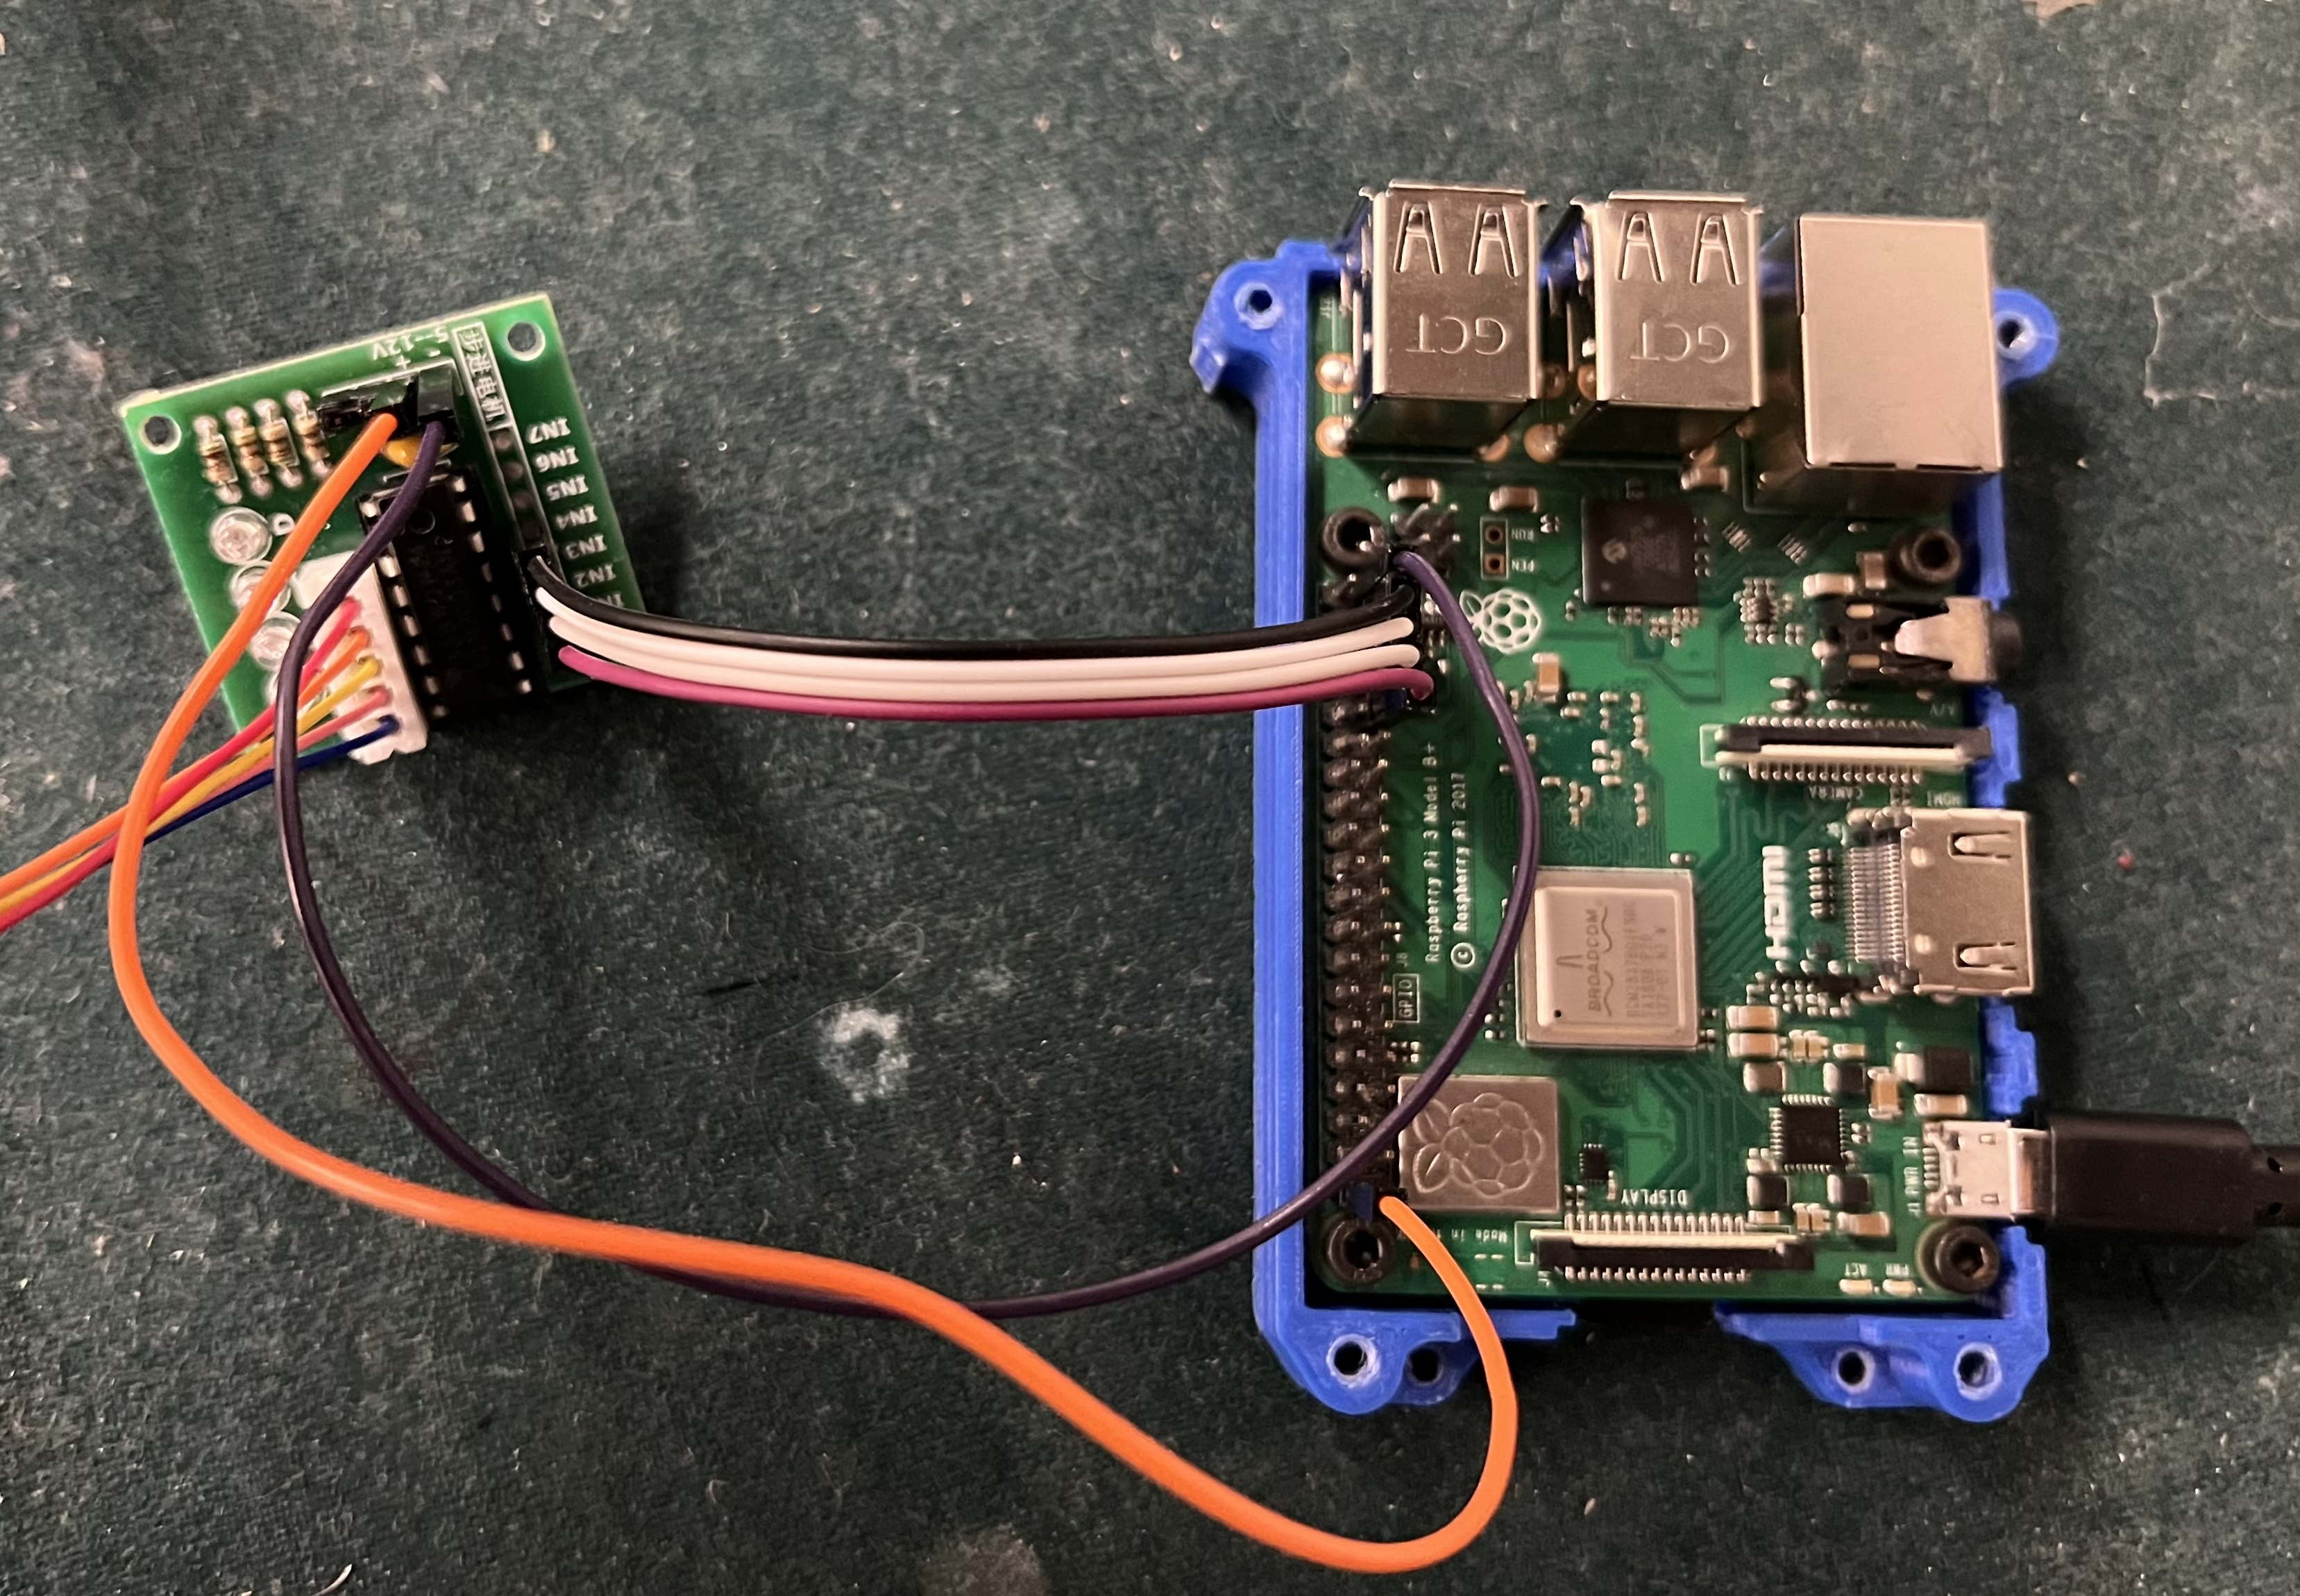
\includegraphics[width=\linewidth]{figures/RaspberryPi_Motor Wiring_Diagram.jpg}
        \caption{Raspberry Pi Motor Wiring Diagram}
        \label{Wiring Diagram}
    \end{minipage}
    \hfill
    \begin{minipage}{0.24\textwidth}
        \centering
        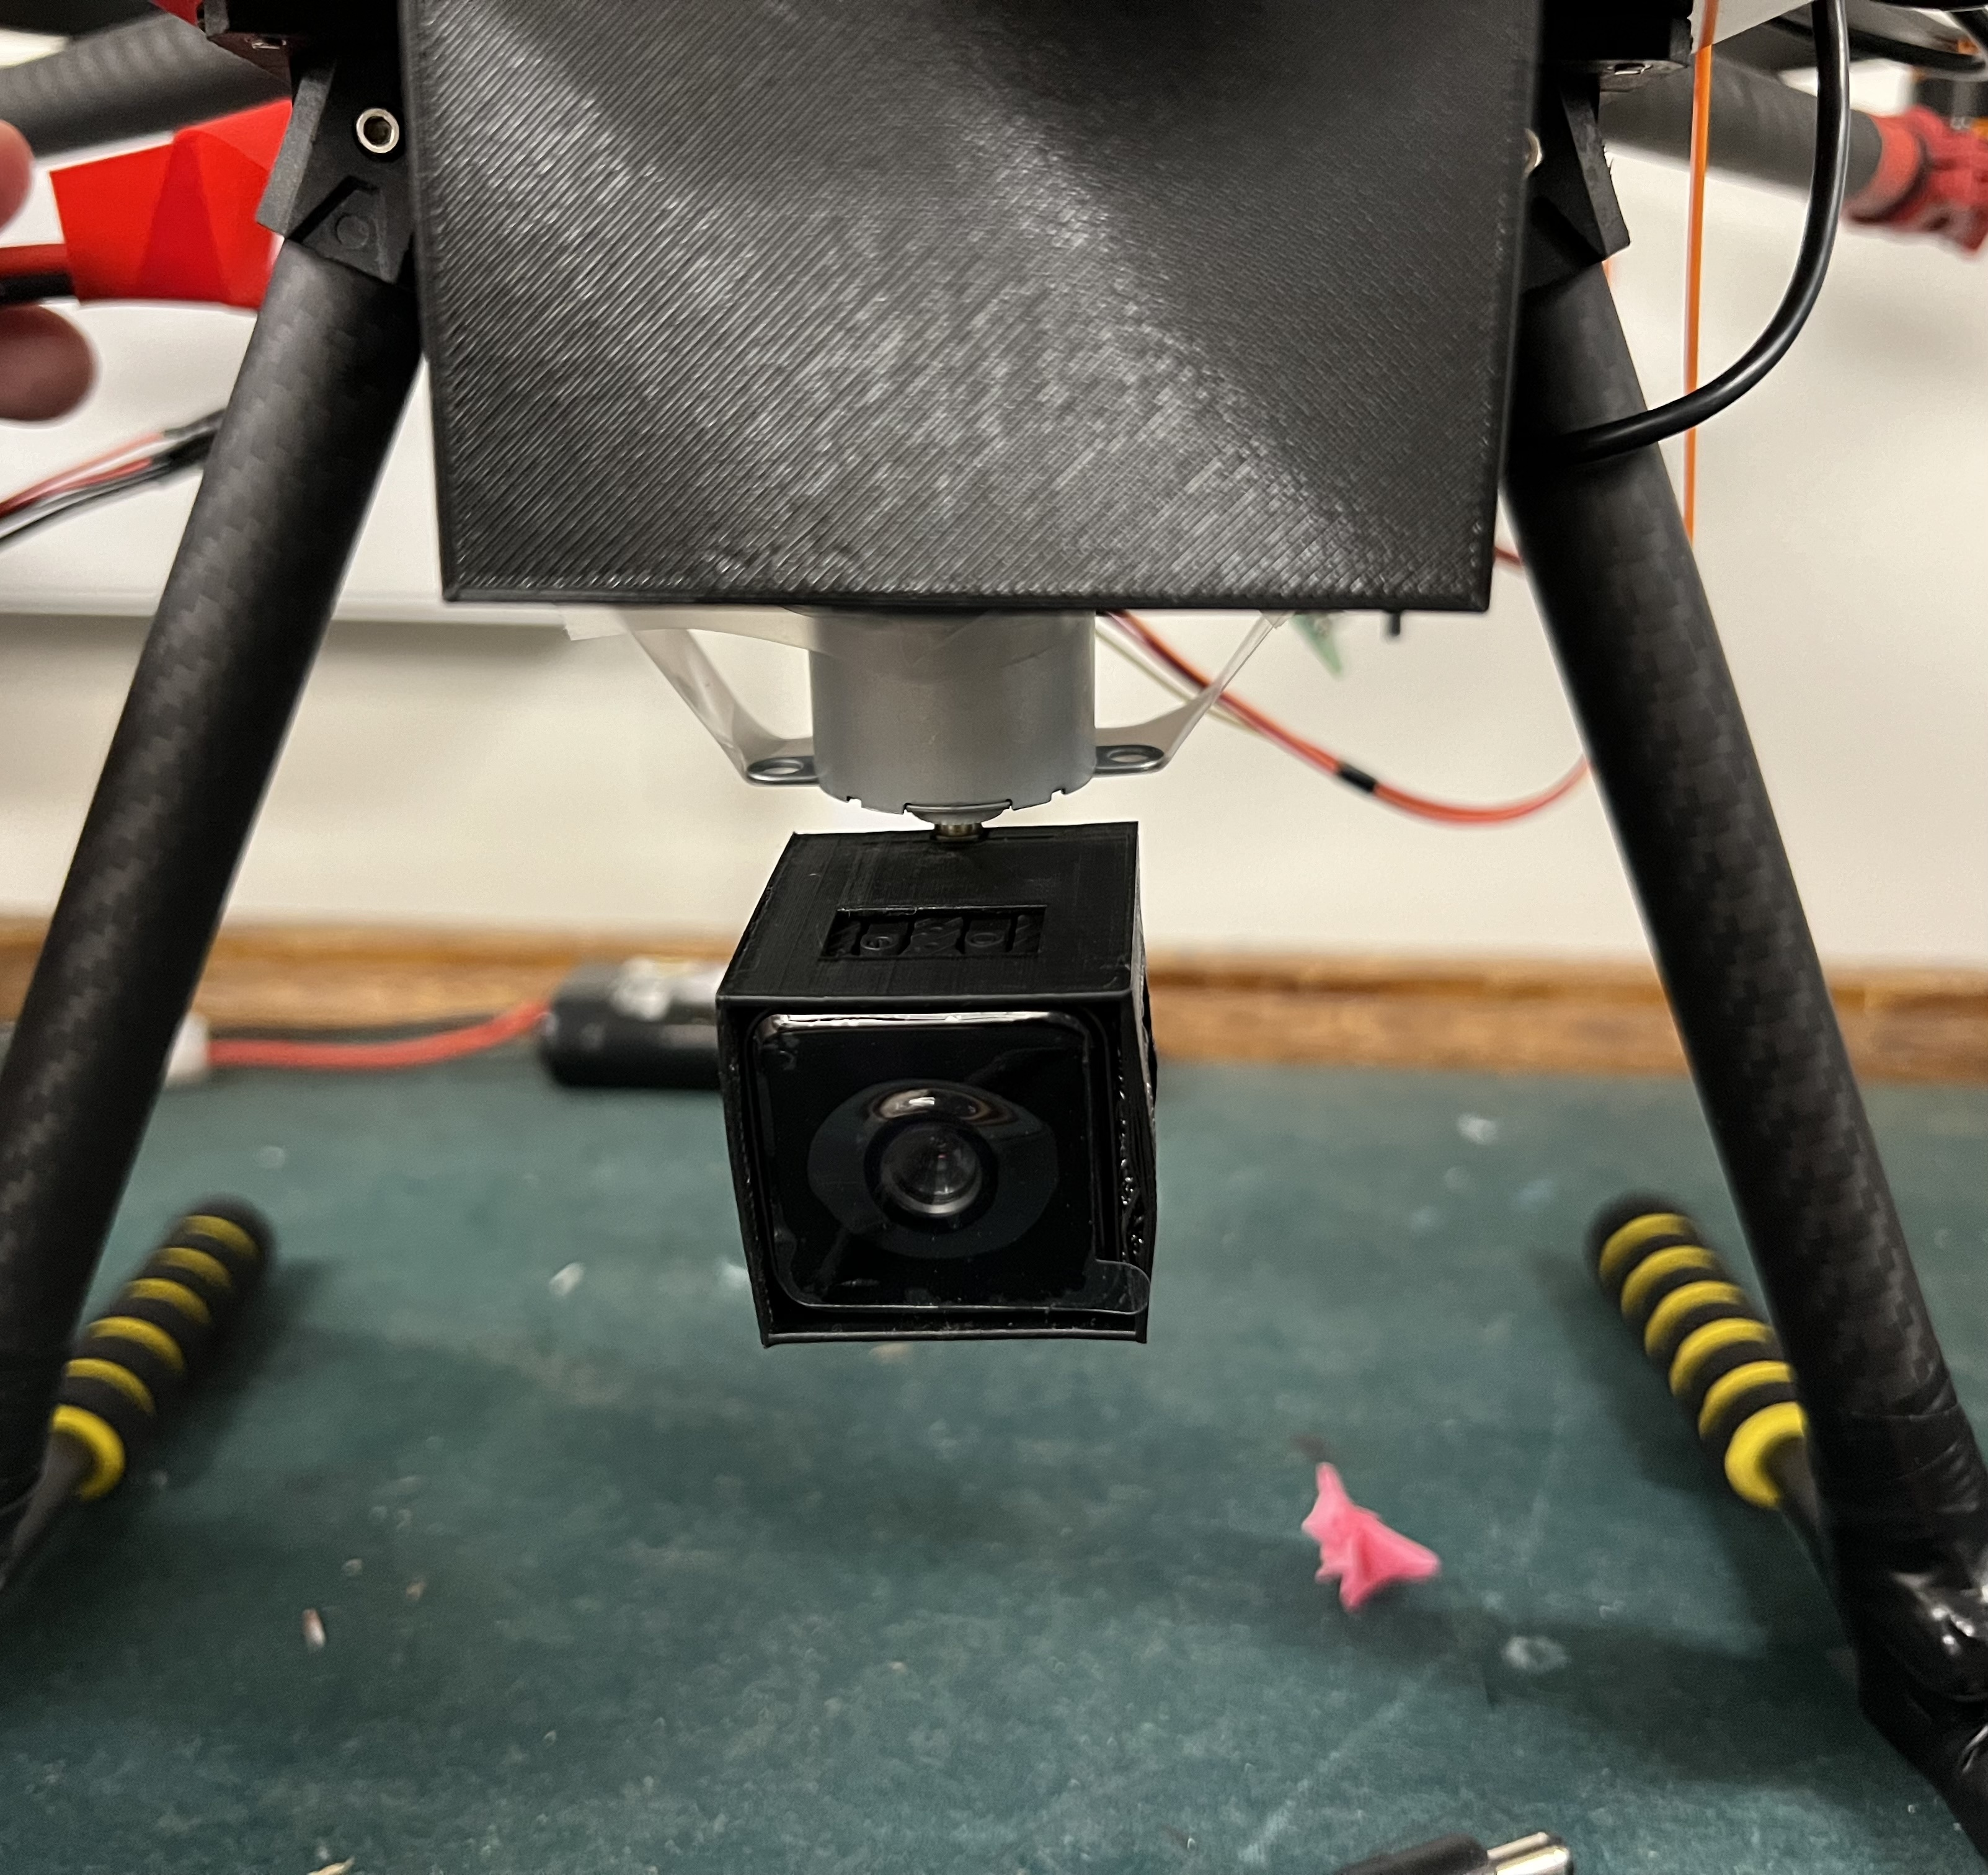
\includegraphics[width=0.8\linewidth]{figures/camera_system.jpg}
        \caption{Camera System}
        \label{camera_system}
    \end{minipage}
\end{figure}

The stepper motor, controlled by a Raspberry Pi through its control lines, has exhibited precise and reliable rotation of the camera assembly\ref{Wiring Diagram}. By establishing an SSH connection between a laptop and the Raspberry Pi, we have remotely controlled the camera's rotation, allowing for a comprehensive view of the environment in real-time\ref{camera_system}.

The initial implementation utilized a compact, off-the-shelf wireless monitoring camera with built-in transmission functionality. This camera has proven effective in capturing and transmitting high-quality video footage to the operator's laptop or control station. The plug-and-play nature of this camera has greatly simplified the implementation process, enabling us to focus on integrating the rotational mechanism.

Throughout our testing, the 360-degree rotational camera system has consistently provided a stable and clear video feed, allowing operators to monitor the drone's surroundings effectively. The system has demonstrated its ability to rotate smoothly and accurately, responding to the operator's commands without noticeable delay or lag.

We have conducted various tests to assess the system's performance in different scenarios, such as indoor and outdoor environments, varying lighting conditions, and different altitudes. The results have shown that the camera system maintains its functionality and video quality across a wide range of operating conditions.

Looking ahead, we plan to further enhance the system by replacing the off-the-shelf camera with a high-resolution camera. This upgrade will allow for even better image quality and the ability to capture detailed images for analysis. Additionally, we aim to explore integrating advanced image processing techniques, such as object detection and tracking, to expand the system's capabilities further.

\subsection{Wireless}
\subsubsection{Jetson Nano}
 Once the necessary software was configured to run on the Jetson Nano, we validated that the drone's battery system was sufficient to supply power to the 5G module through the Nano while still powering the drone and the other sensors within the drone's payload. Both the RM502Q-AE and the RM520N-GL were validated for power and interface creation. Interface creation was used to validate the environment because it validated that the Jetson Nano could manipulate the module through AT Commands and drivers were properly installed for serial use and interface management. 
\subsubsection{RM520N-GL}
While not our first choice for part of the payload, we achieved a significant measure of success by using the RM520N-GL module to establish a data session with the 5G Network. While connected to the drone, we established a data session that allowed us to send and receive ICMP traffic between the Nano and the Core Network as seen in Figure 8 and 9. 
\begin{figure}[htbp]
    \centering
    \resizebox{9cm}{5cm}
    {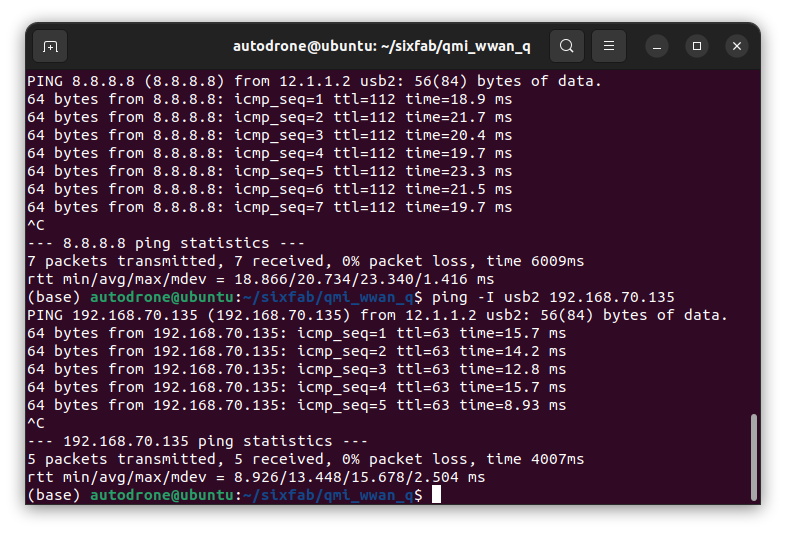
\includegraphics{figures/ICMP_nano.png}}
    \caption{ICMP Packets on the Nano to the Core Network}
    \label{icmp nano}
\end{figure}
\begin{figure}[htbp]
    \centering
    \resizebox{9cm}{5cm}
    {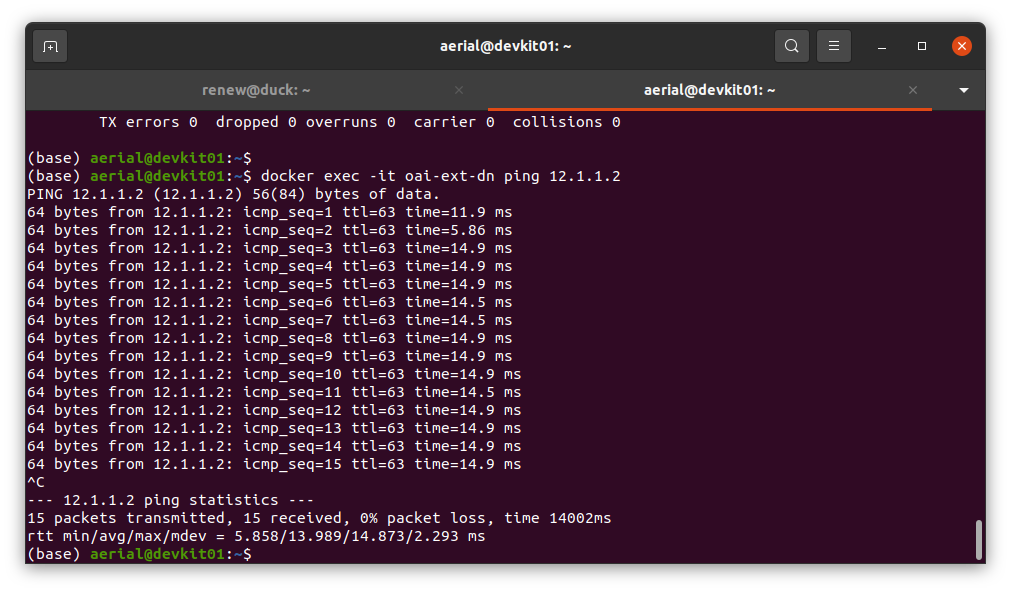
\includegraphics{figures/ICMP_core.png}}
    \caption{ICMP Packets from Server on the Core Network to the Nano}
    \label{icmp nano}
\end{figure}
\subsubsection{RM505Q-AE}
Throughout testing, the RM502Q-AE has not established a data session with the 5G network. Despite this, we were successful in validating the module in both the testing and operational environment which supports the suitability of the module for the drone once resolved. We were also able to incorporate the success of the RM520N-GL by using it as baseline to compare configurations and behavior with the Core Network, L1 and L2. Specifically, we were able to validate the SIM card we configured for the RM502Q-AE by using that SIM card with the RM502Q-AE to establish a successful data session. We verified that the module itself as well as the network recognized the different SIM cards by matching the IMSI in the logs during UE Registration as seen in the figure below. 
\begin{figure}[htbp]
    \centering
    \resizebox{9cm}{5cm}
    {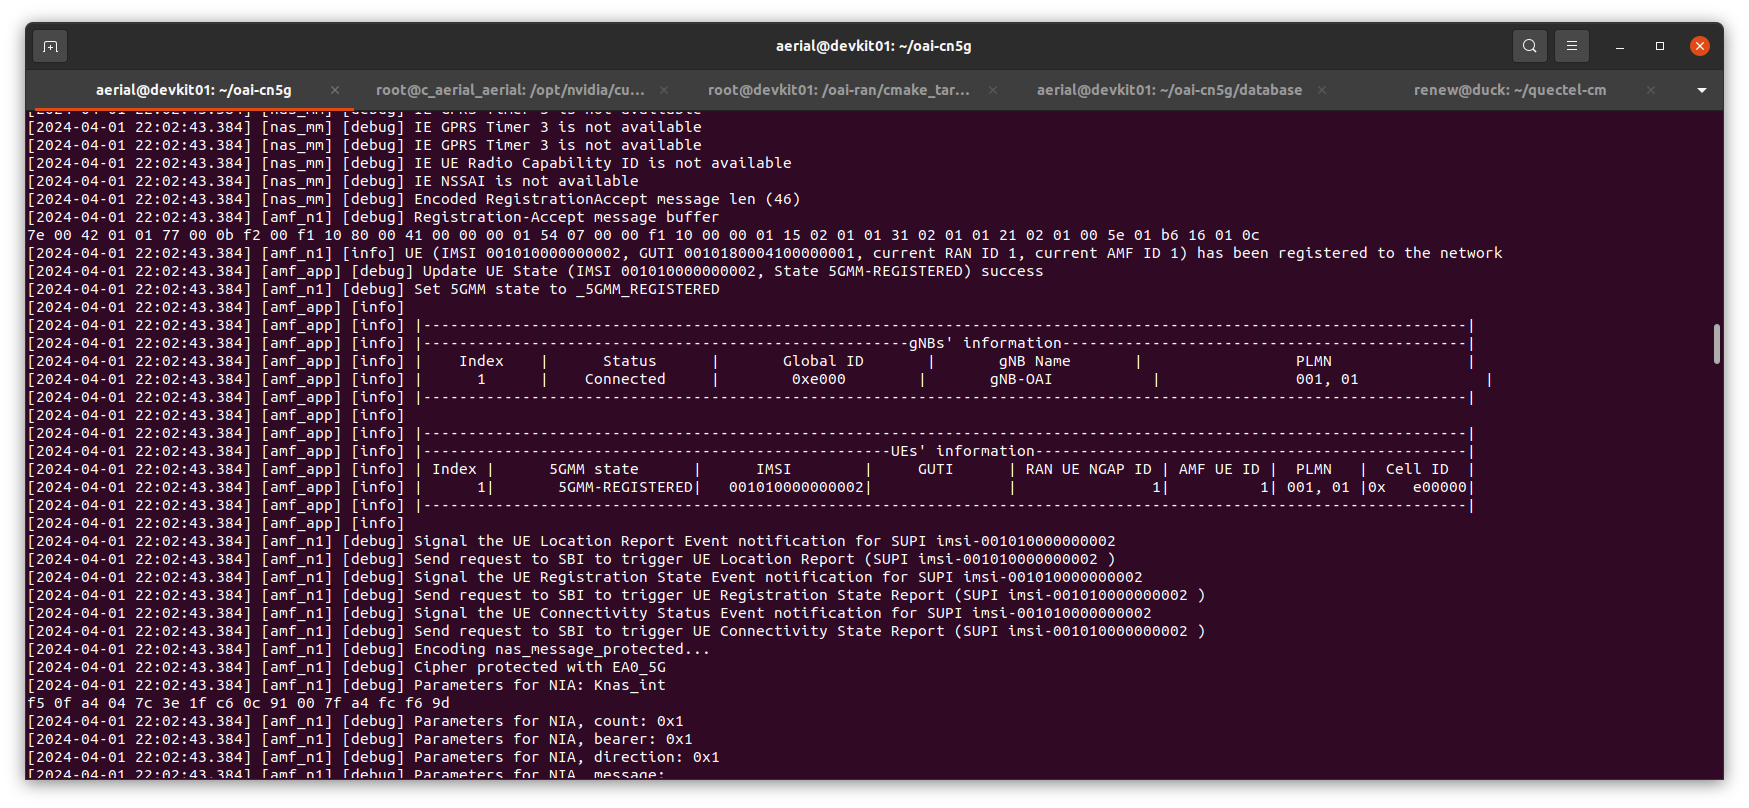
\includegraphics{figures/registeredIMSI.png}}
    \caption{UE Registration on Network with UE IMSI}
    \label{IMSI Registered}
\end{figure}

\subsection{Object Detection}
\subsubsection{Algorithm Comparison and ROS2 Integration}
\paragraph{Testing on VisDrone Dataset}
Initial evaluations on a laptop webcam identified the single-stage detector YOLOv8 as the most optimal choice for real-time object detection among FasterRCNN, RetinaNet, YOLOv5, and YOLOv8. Given the need for highly efficient real-time performance on autonomous drones, we focused our subsequent testing on single-stage object detectors by evaluating RetinaNet, YOLOv8, and the newly proposed YOLOv9 on the VisDrone dataset. 

Experiments were conducted to evaluate the accuracy and speed of each algorithm using metrics such as mean Average Precision (mAP) and Frames Per Second (FPS). The experiments involved testing the algorithms on a diverse set of real-life scenarios captured in the VisDrone dataset using an NVIDIA A100 GPU. Table \ref{performances} presents a summary of the performances achieved by the trained models. Additionally, Figure \ref{comparison_training} depicts the mAP values of YOLOv8, YOLOv9, and its extension on the training set across the training process.

\begin{table}[h]
\begin{center}
\begin{tabular}{ |c|c|c|c| } 
 \hline
 Model (trained) & mAP50 & mAP50-95 & FPS \\ 
 \hline
 RetinaNet & 0.537 & 0.313 & 5 \\ 
 \hline
 YOLOv8 & 0.335 & 0.195 & 18.35 \\ 
 \hline
 YOLOv9 & 0.458 & 0.285 & 20.83 \\
 \hline
 YOLOv9-e & 0.471 & 0.299 & 13.35 \\
 \hline
\end{tabular}
\end{center}
\caption{Performances of Trained Models in VisDrone}
\label{performances}
\end{table}

\begin{figure}[htbp]
    \centering
    \resizebox{9cm}{5cm}
    {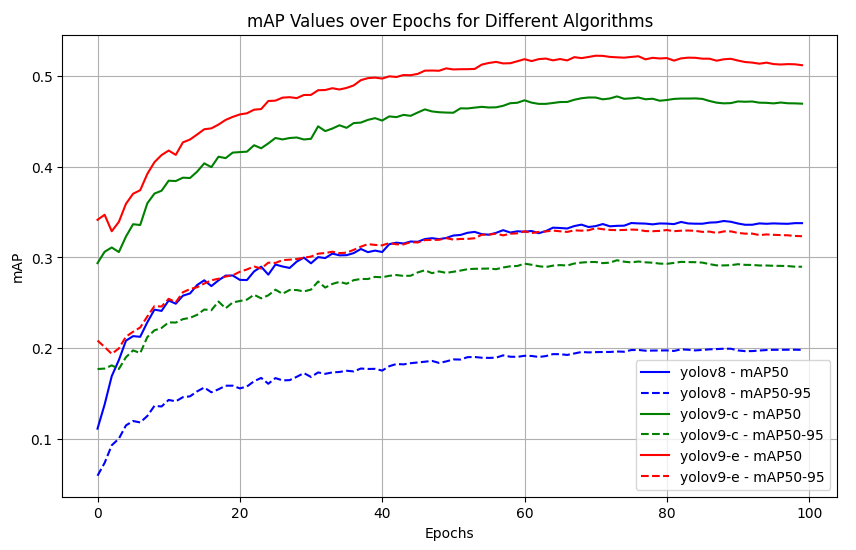
\includegraphics{figures/yolov8_vs_yolov9.png}}
    \caption{mAP Values vs Training Epochs}
    \label{comparison_training}
\end{figure}

Results showcased RetinaNet's impressive accuracy albeit at a slower speed compared to YOLOv9. Notably, YOLOv9 demonstrated enhancements in both accuracy and speed over YOLOv8. While YOLOv9 extension model had higher accuracy than YOLOv9, it is even slower than YOLOv8. The results of the study underscored the superiority of YOLOv9 as the preferred real-time object detection model for the autodrone project. 

\paragraph{Testing on Gazebo}
YOLOv8l and YOLOv9 were chosen for comparison in Gazebo simulation as they exhibited similar mean Average Precision (mAP) values on MS COCO dataset, as shown in Table \ref{Comparison}. This allowed for a fair evaluation of their speed performance while ensuring comparable accuracy levels. Initial tests were conducted on a CPU, specifically an Intel Core i7. YOLOv9 demonstrated an average inference time of 816.8ms per image, outperforming YOLOv8l by 23\% as the latter exhibited 1004.3ms inference time. Subsequently, the algorithms were evaluated on an Nvidia GeForce RTX 3070 GPU. The average inference time of YOLOv8l was 13.4ms, while YOLOv9 achieved an average of 10.6ms, indicating that YOLOv9 is approximately 26\% faster than YOLOv8l when leveraging GPU acceleration. Comparative analyses on different hardware configurations reaffirmed YOLOv9's advantages, with significant improvements in inference times observed.

\begin{table}[h]
\begin{center}
\begin{tabular}{ |c|c|c|c|c|c| } 
 \hline
 Model  & mAP50-95 & Param. & FLOPs & FPS (CPU) & FPS (GPU) \\ 
 \hline
 YOLOv8l & 0.529 & 43.7M & 165.2G & 1.0 & 74.6 \\ 
 \hline
 YOLOv9  & 0.530 & 25.3M & 102.1G & 1.2 & 94.3\\ 
 \hline
\end{tabular}
\end{center}
\caption{Performances of YOLOv8l and YOLOv9 in Gazebo Simulation}
\label{Comparison}
\end{table}

The successful integration of YOLOv9 into the ROS2 environment further validated its suitability for real-world deployment scenarios. ROS2's enhanced capabilities, including improved adaptability to diverse environments and superior visual quality in Gazebo simulations, complemented YOLOv9's performance, paving the way for future developments and live tests with the auto-drone platform.

Overall, the findings highlight YOLOv9 as a promising solution for real-time object detection in autonomous drone applications, with potential implications for enhancing efficiency and safety in various industries and domains. 
\subsubsection{TensorRT Acceleration}

It's crucial to create benchmarks on dataset to evaluate performance. Once the model converted by TensorRT to run inference, it's noticeable that it significantly enhances the performance on COCO128 in terms of speed compared to PyTorch and TorchScript, with YOLOv8x showing the most substantial improvement, as shown in figure\ref{TensorRT}.
\begin{figure}[htbp]
    \centering
    \resizebox{9cm}{4cm}
    {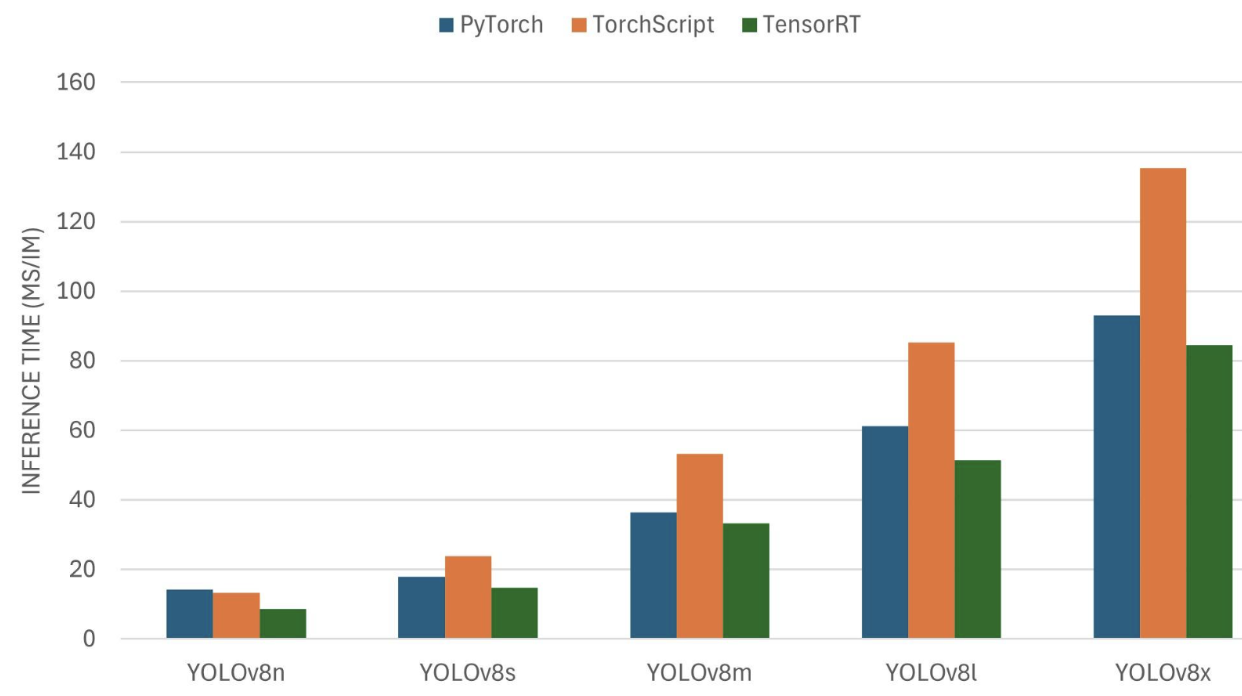
\includegraphics{figures/tensor.png}}
    \caption{TensorRT Acceleration on Yolov8}
    \label{TensorRT}
\end{figure}
\subsection{3D Reconstruction}
\subsubsection{Datasets}
We first validate our method with TUM~\cite{tum} and MipNerf-360~\cite{mipnerf360} dataset. These two datasets, TUM, are commonly used for indoor SLAM testing; NERF360 is commonly used for evaluating the quality of implicit 3D representations. Additionally, we also use the drone to collect some real-world data at Rice University.
\subsubsection{3D Gaussian Splatting}
We perform Gaussian Splatting on the three mentioned dataset. Fig. \ref{gaussian_result} shows the novel view synthesis results.

\begin{figure}[htbp]
    \centering
    \resizebox{9cm}{5cm}
    {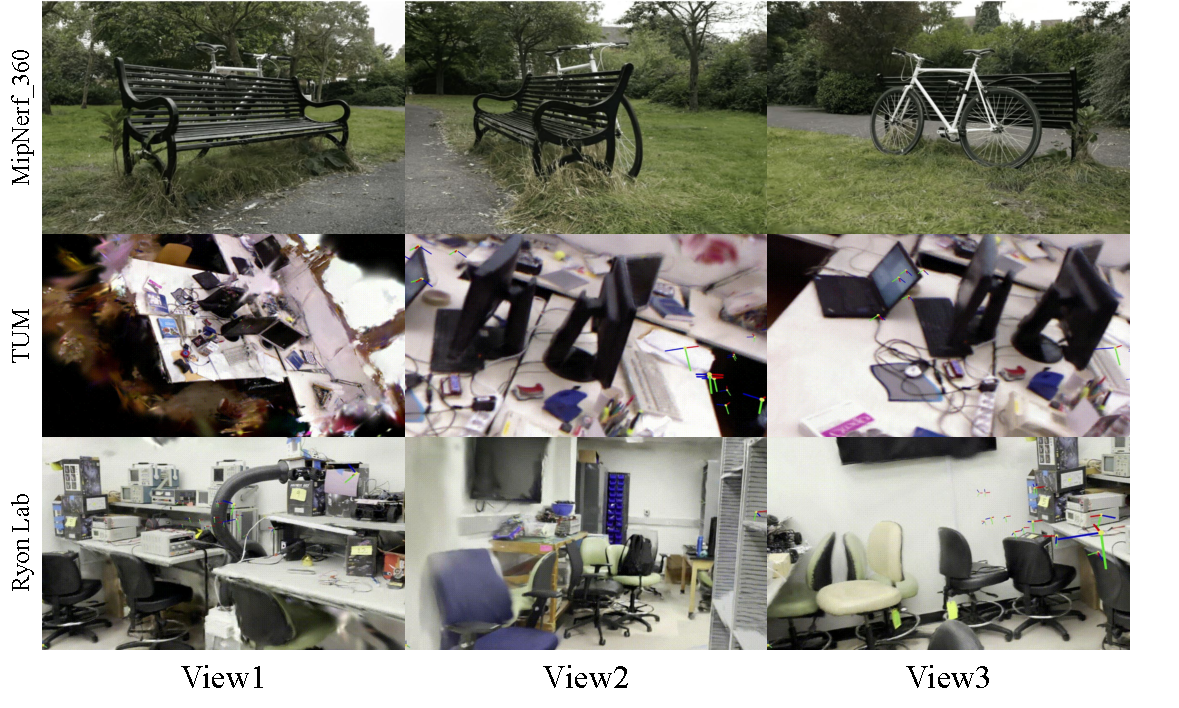
\includegraphics{figures/3dgs_recon.pdf}}
    \caption{3D Gaussian Splatting results on the MipNerf-360, TUM and our collected Ryon lab data. We selected 3 different views and three scene from our trained Gaussian fields. The frames in the images denote the training input camera frame positions.}
    \label{gaussian_result}
\end{figure}

Further, we compare the original Gaussian Splatting pipeline with our depth supervised version on the TUM dataset. As shown in Fig.~\ref{gaussian_depth}, the edges of the window were quite blurry, but after adding depth constraints, they become cleaner and closer to the ground truth. Additionally, we conduct quantitative evaluations as shown in Table \ref{tab:psnr}. 
\begin{figure}[htbp]
    \centering
    \resizebox{9cm}{5cm}
    {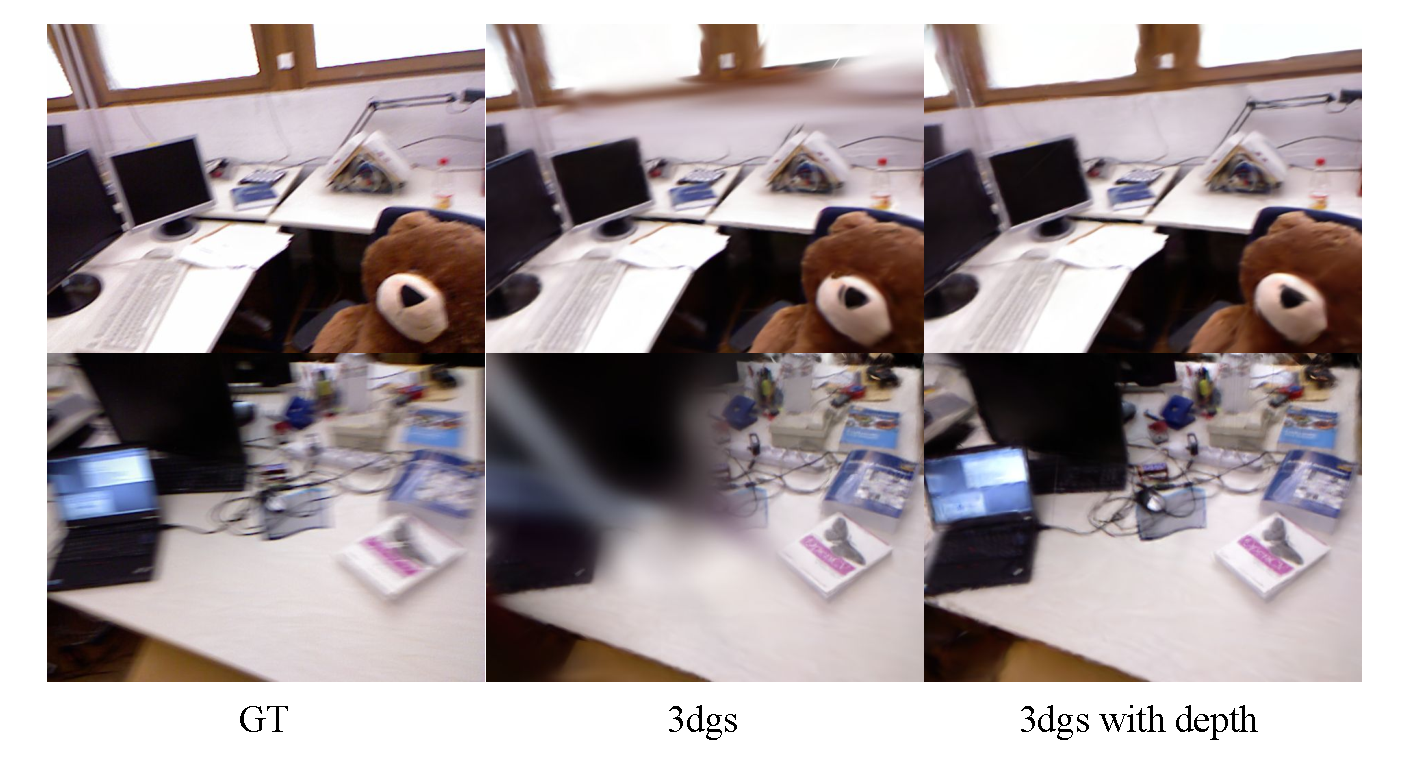
\includegraphics{figures/gaussian_depth.pdf}}
    \caption{We apply depth constraint during training 3D Gaussians. Depth loss between the rendered depth and ground truth depth help optimizing Gaussians' position attributes. The depth supervised results display cleaner reconstruction and sharper edges.}
    \label{gaussian_depth}
\end{figure}
We choose to report the PSNR metrics within the training set. Depth constraint has improved the representation quality in terms of PSNR, which however, is not too obvious.

\begin{table}[htbp]
\centering
\begin{tabular}{@{}ll@{}}
\toprule
\textbf{Methods} & \textbf{PSNR} \\ 
\midrule
Original 3DGS &  24.608657836914062\\ 
3DGS with depth &  24.7428035736084\\ 
3DGS with depth (larger positional lr) &  24.92386817932129\\ 
\bottomrule
\end{tabular}
\caption{PSNR Metrics}
\label{tab:psnr}
\end{table}

\subsubsection{Camera-Lidar Fusion}
Optical images from the camera provide rich texture and color details, while LiDAR data offers precise depth information and structural insights. Three distinct images demonstrate the capabilities of this system. As shown in Fig.\ref{lzn},the left part captures the real scene as viewed by the fusion system, illustrating how it merges visual and depth data for a detailed environmental view. The mid part is a 3D point cloud generated from LiDAR data, representing the environment's spatial structure,while the right part shows a rendered view where LiDAR points are colorized using corresponding pixels from the camera image, resulting in a vivid and detailed 3D representation that marries structural integrity with visual realism. This comprehensive approach improves data accuracy and enriches the environment's visual representation, proving essential for precise and realistic modeling.
\begin{figure}[htbp]
    \centering
    \resizebox{9cm}{2cm}
    {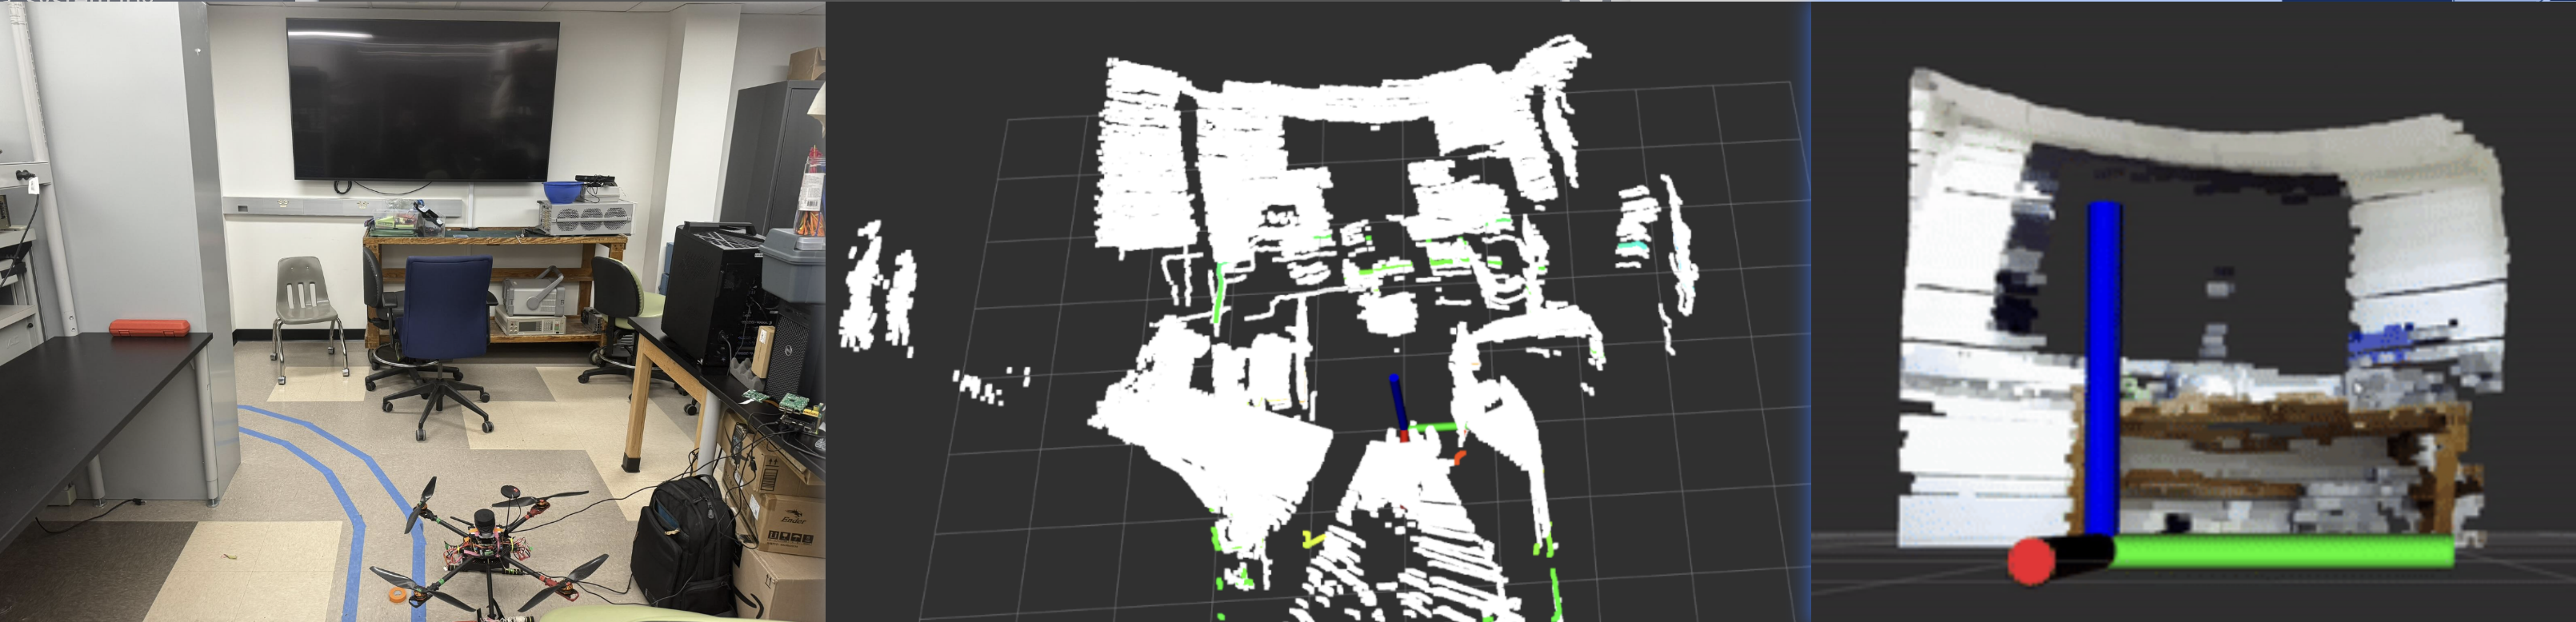
\includegraphics{figures/lzn.png}}
    \caption{Real World Scene and 3d pointcloud}
    \label{lzn}
\end{figure}


\subsubsection{Object Extraction}
We test our extraction approach on the MipNerf-360 garden dataset and result in the 3D Gaussians of the vase as shown in the top right part of Fig.~\ref{extraction}. The background is successfully removed. We find that sifting out background point cloud before training Gaussians is important for clean removal.
\begin{figure}[htbp]
    \centering
    \resizebox{9cm}{5cm}
    {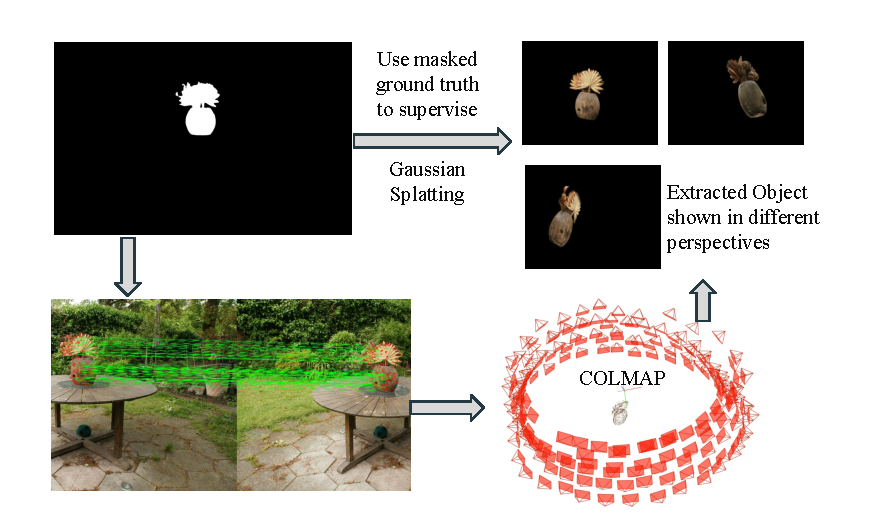
\includegraphics{figures/Extraction.pdf}}
    \caption{The 3D object Extraction pipeline and the result. Our task is to reconstruct the vase without the background. The masks are used for both key points screening and raterization screening. }
    \label{extraction}
\end{figure}
\section{Discussion}
We have developed our auto-drone product in several aspects, including hardware improvement, wireless connections and vision algorithms. Our long term goal is to equip the drone with strong ability to identify people and survey environment, towards which we are making small but important steps. 

However, our current solutions still have limitations. In terms of 3D reconstruction, we observe that when the lighting is unstable or texture is poor (indoor environment), 3D Gaussian Splatting reconstruction quality is largely compromised. Even though we have applied depth constraint during reconstruction, the position of gaussians are more influenced by the initial point clouds. As a result, Gaussian field trained with depth still contains many floaters. Further investigations are needed before we combine the pipeline with Lidar data. Furthermore, both the reconstruction and detection algorithm require substantial computation, which limit their direct implementation on the drone. We might need to consider developing fast and stable data transmission between the drone and the station. Otherwise, these algorithms can only be carried out offline.



\section{Conclusion}
In conclusion, our work showcases the innovative integration of advanced hardware and software technologies to enhance the operational efficiency and safety of first responders in hazardous environments. The development of an autonomous drone equipped with a 360-degree camera, optimized object detection algorithms like YOLOv9, and the incorporation of 3D reconstruction techniques represent significant technological advancements.

% The use of Gaussian splatting for 3D environmental modeling, along with the effective implementation of ROS2 for simulation and real-world application, underscores the project's cutting-edge nature. The system's ability to perform under diverse conditions and its potential for real-time applications highlight its practical relevance and potential impact on emergency response strategies.

While the project has achieved remarkable results, ongoing efforts to refine the drone's capabilities and ensure its reliability across various scenarios are crucial. The continuous evolution of the drone's design and functionality is aimed at meeting the rigorous demands of real-world emergency response operations. The collaboration and contributions of a multidisciplinary team have been pivotal in navigating the challenges associated with this complex project.

This project not only demonstrates the feasibility of using autonomous drones for challenging environments but also sets a benchmark for future research and development in the field of autonomous emergency response systems. The learnings from this project can guide similar initiatives, aiming to harness the power of advanced technology to safeguard lives in critical situations.


\section*{Acknowledgements}
This research was made possible by the generous financial support from the Rice University Electrical and Computer Department, to whom we extend our heartfelt gratitude.

We owe a profound debt of gratitude to Dr. Joseph Young, our mentor for the Autodrone project, for his invaluable guidance and expert advice throughout the duration of this project. On behalf of the entire team, we also extend our heartfelt thanks to Dr. Rahman Doost for his invaluable support and expertise in 5G communications, which greatly enhanced our project. Our sincere thanks also go to the former members of the Autodrone project, whose pioneering work laid the groundwork for our research. Their contributions have been instrumental in achieving the outcomes presented in this study.



% Please number citations consecutively within brackets \cite{b1}. The 
% sentence punctuation follows the bracket \cite{b2}. Refer simply to the reference 
% number, as in \cite{b3}---do not use ``Ref. \cite{b3}'' or ``reference \cite{b3}'' except at 
% the beginning of a sentence: ``Reference \cite{b3} was the first $\ldots$''

% Number footnotes separately in superscripts. Place the actual footnote at 
% the bottom of the column in which it was cited. Do not put footnotes in the 
% abstract or reference list. Use letters for table footnotes.

% Unless there are six authors or more give all authors' names; do not use 
% ``et al.''. Papers that have not been published, even if they have been 
% submitted for publication, should be cited as ``unpublished'' \cite{b4}. Papers 
% that have been accepted for publication should be cited as ``in press'' \cite{b5}. 
% Capitalize only the first word in a paper title, except for proper nouns and 
% element symbols.

% For papers published in translation journals, please give the English 
% citation first, followed by the original foreign-language citation \cite{b6}.

\begin{thebibliography}{00}
\bibitem{stepper} T. Kenjo and A. Sugawara, Stepping Motors and Their Microprocessor Controls. Oxford, U.K.: Oxford University Press, 2003.
\bibitem{rasp}  Y. Lai, "Stepper Motor Control In Python Using Raspberry Pi GPIO," Medium, Nov. 26, 2017. [Online]. Available: https://medium.com/@yik.lai/raspberry-pi-stepper-motor-control-in-python-using-pigpio-66a43fc99870. 
\bibitem{3dgs} Kerbl, Bernhard, et al. "3d gaussian splatting for real-time radiance field rendering." ACM Transactions on Graphics 42.4 (2023): 1-14.
\bibitem{colmap}Schonberger, Johannes L., and Jan-Michael Frahm. "Structure-from-motion revisited." Proceedings of the IEEE conference on computer vision and pattern recognition. 2016.
\bibitem{ransac}Chum, Ondřej, Jiří Matas, and Josef Kittler. "Locally optimized RANSAC." Pattern Recognition: 25th DAGM Symposium, Magdeburg, Germany, September 10-12, 2003. Proceedings 25. Springer Berlin Heidelberg, 2003.
\bibitem{tum}Sturm, Jürgen, et al. "A benchmark for the evaluation of RGB-D SLAM systems." 2012 IEEE/RSJ international conference on intelligent robots and systems. IEEE, 2012.
\bibitem{mipnerf360}Barron, Jonathan T., et al. "Mip-nerf 360: Unbounded anti-aliased neural radiance fields." Proceedings of the IEEE/CVF Conference on Computer Vision and Pattern Recognition. 2022.
\bibitem{FasterRCNN}Ren, Shaoqing, Kaiming He, Ross Girshick, and Jian Sun. "Faster r-cnn: Towards real-time object detection with region proposal networks." Advances in neural information processing systems 28 (2015).
\bibitem{RetinaNet}Lin, Tsung-Yi, Priya Goyal, Ross Girshick, Kaiming He, and Piotr Dollár. "Focal loss for dense object detection." In Proceedings of the IEEE international conference on computer vision, pp. 2980-2988. 2017.
\bibitem{YOLOv5}Ultralytics, "YOLOv5: A state-of-the-art real-time object detection system", https://docs.ultralytics.com. 2021.
\bibitem{YOLOv8}Jocher, G., Chaurasia, A., & Qiu, J. (2023). Ultralytics YOLO (Version 8.0.0) [Computer software]. https://github.com/ultralytics/ultralytics
\bibitem{YOLOv9}Wang, Chien-Yao, I-Hau Yeh, and Hong-Yuan Mark Liao. "YOLOv9: Learning What You Want to Learn Using Programmable Gradient Information." arXiv preprint arXiv:2402.13616. 2024.
\bibitem{sam}Kirillov, Alexander, et al. "Segment anything." Proceedings of the IEEE/CVF International Conference on Computer Vision. 2023.
\bibitem{dino}Liu, Shilong, et al. "Grounding dino: Marrying dino with grounded pre-training for open-set object detection." arXiv preprint arXiv:2303.05499 (2023).
\bibitem{visdrone}{Zhu, Pengfei,et al."Detection and tracking meet drones challenge",IEEE Transactions on Pattern Analysis and Machine Intelligence}
\end{thebibliography}
\vspace{12pt}


\end{document}
